\chapter{Implementação da Solução}
\label{cap:implementação}

Neste capítulo descreve-se a implementação do backoffice multiaplicação, apresentando as soluções técnicas adotadas e evidências do trabalho desenvolvido. A JustCauses é a primeira aplicação operacional integrada e, por isso, recebe maior detalhe funcional. A estrutura do capítulo começa pelos módulos transversais ao ecossistema, como autenticação, controlo de acesso, gestão de operadores e auditoria, e depois descreve os módulos operacionais da JustCauses. No final, são apresentados os testes e a avaliação da solução, separando a descrição do que foi implementado da análise sobre como esse trabalho foi validado.

%----------------------------------------------------------------------------------------

\section{Ambiente e estrutura do projeto}
\label{sec:ambiente_infraestrutura}

O repositório está organizado em duas pastas raiz independentes: \texttt{be/} para o \textit{back-end} e \texttt{fe/} para o \textit{front-end}, cada uma com a sua configuração de dependências e de compilação. O \textit{back-end} arranca com \texttt{ts-node} em modo de desenvolvimento e compila para JavaScript em produção; o \textit{front-end} usa o servidor de desenvolvimento do Vite com \textit{Hot Module Replacement}. O controlo de versões segue uma estratégia de \textit{branching} com ramos de funcionalidade (\texttt{feature/*}) e revisão de código por \textit{pull request} antes da integração no ramo principal.

A injeção de dependências no \textit{back-end} é configurada no ficheiro \texttt{be/src/loaders/index.ts}, que regista todos os repositórios, serviços e controladores no contentor do TypeDI antes de o Express montar as rotas. Esta separação garante que as dependências são resolvidas em tempo de arranque e não em tempo de pedido, evitando instanciações desnecessárias.

A entrega para o ambiente de desenvolvimento está parcialmente automatizada com Bitbucket Pipelines, em fluxos separados para o \textit{front-end} e para o \textit{back-end}. No \textit{front-end}, cada atualização ao ramo \texttt{developer} instala as dependências, executa a \textit{build} com Vite, publica a pasta \texttt{dist/} num \textit{bucket} Amazon S3 dedicado ao ambiente de desenvolvimento e invalida a distribuição CloudFront para garantir a propagação imediata dos novos \textit{assets}. No \textit{back-end}, o pipeline constrói uma imagem Docker da aplicação, autentica-se no Amazon ECR através da AWS CLI, aplica uma etiqueta imutável baseada em \textit{timestamp} UTC e publica tanto essa versão como a etiqueta \texttt{latest}. Esta separação permitiu iterar a interface e a \gls{API} com ritmos diferentes sem introduzir acoplamento desnecessário no processo de entrega.

%----------------------------------------------------------------------------------------

\section{Autenticação e controlo de acesso}
\label{sec:autenticacao_impl}

A autenticação é gerida pelo AWS Cognito com o fluxo OAuth 2.0 / JWT padrão. No entanto, o elemento central da implementação não é apenas o \textit{login}; é a sequência de decisões que ocorre depois: identificar o operador, determinar a que aplicação pode aceder, definir que páginas pode abrir e decidir que pedidos o \textit{back-end} deve aceitar ou rejeitar. Para tornar este mecanismo mais claro, a sua implementação é descrita aqui por passos.

\subsection{Passo 1: autenticar e resolver o contexto do operador}
\label{subsec:auth_step1}

No \textit{front-end}, a sessão é gerida pelo AWS Amplify. Depois de uma autenticação bem-sucedida, o \texttt{AuthProvider} não fica apenas com os dados básicos devolvidos pelo Cognito. Faz também um pedido ao endpoint \texttt{/users/me} para obter o contexto interno do operador: identificador no backoffice, perfis atribuídos, aplicações acessíveis, permissões efetivas e permissões agrupadas por aplicação. Esta segunda leitura é necessária, porque o token Cognito identifica a sessão, mas não descreve sozinho as regras de autorização do painel.

No \textit{back-end}, esse contexto é montado no \textit{middleware} \texttt{cognitoAuth.ts}. O token Bearer é validado contra o \textit{JWKS} público do Cognito, o \texttt{token\_use} tem de ser \texttt{access}, o \texttt{client\_id} tem de coincidir com a configuração da aplicação e o \texttt{sub} do Cognito é usado para localizar o operador na base de dados interna. Só depois disso o sistema resolve os perfis guardados em \texttt{roleIds}, lê as permissões disponíveis e calcula o acesso efetivo através de uma função central. O resultado é anexado a \texttt{req.auth}, incluindo \texttt{roles}, \texttt{permissions}, \texttt{permissionsByApplication}, \texttt{appsAccessible} e \texttt{isSuperAdmin}. Se a conta não existir no backoffice ou estiver desativada, o pedido é rejeitado logo neste ponto.

O excerto da Listagem~\ref{lst:effective_access} mostra o ponto onde a autorização passa a depender também da aplicação associada a cada perfil e a cada permissão.

\begin{lstlisting}[caption={Excerto do cálculo do acesso efetivo por aplicação}, label={lst:effective_access}]
const backofficeRole =
  roles.find(role => role.application === "backoffice") ?? null;
const isSuperAdmin =
  roles.some(role => role.name === SUPER_ADMIN_ROLE_NAME);

if (isSuperAdmin) {
  allPermissions.forEach(permission =>
    addPermission(permissionsByApplicationSets, permission),
  );
} else if (backofficeRole) {
  allPermissions
    .filter(permission => permission.application !== "backoffice")
    .forEach(permission =>
      addPermission(permissionsByApplicationSets, permission),
    );

  backofficeRole.permissions.forEach(rolePermission => {
    const permission = permissionByName.get(rolePermission.name);
    if (permission?.application === "backoffice") {
      addPermission(permissionsByApplicationSets, permission);
    }
  });
} else {
  roles.forEach(role => {
    role.permissions.forEach(rolePermission => {
      const permission = permissionByName.get(rolePermission.name);
      if (permission?.application === role.application) {
        addPermission(permissionsByApplicationSets, permission);
      }
    });
  });
}

const permissionsByApplication =
  toPlainPermissions(permissionsByApplicationSets);
\end{lstlisting}

A Listagem~\ref{lst:effective_access} mostra que a autorização é calculada no servidor e devolvida já separada por aplicação. O Super Admin recebe todas as permissões; um perfil de backoffice recebe automaticamente permissões das aplicações operacionais e apenas as permissões administrativas de backoffice que estiverem associadas ao próprio perfil; um perfil aplicacional só recebe permissões da sua aplicação. Assim, uma nova aplicação pode usar o mesmo mecanismo de autenticação e autorização sem criar uma matriz fixa de acessos no cliente.

Há três exceções públicas a esta regra global, relacionadas com verificação de estado da \gls{API}, registo de falhas de autenticação e registo de tentativas de acesso. Mesmo nesses casos, a implementação tenta anexar autenticação opcional quando existe um token, sem bloquear o pedido se ele faltar ou for inválido.

\subsection{Passo 2: decidir o acesso à aplicação e à página}
\label{subsec:auth_step2}

O roteamento protegido do \textit{front-end} está dividido em quatro guardas: \texttt{ProtectedRoute}, \texttt{PublicRoute}, \texttt{BackofficeRoute} e \texttt{PanelRoute}. A diferença relevante está nas duas últimas: uma controla o acesso ao backoffice administrativo e a outra controla o acesso ao painel operacional pedido, neste caso a JustCauses. Quando a aplicação é recusada, a interface apresenta um ecrã de acesso negado e envia, em segundo plano, um registo de tentativa falhada.

Depois de entrar na aplicação certa, o sistema ainda tem de decidir a que página encaminhar o operador. Essa decisão é feita duas vezes. Primeiro, no \textit{router}, através das listas \texttt{PANEL\_PAGES} e \texttt{ADMIN\_PAGES}, que definem a permissão base de cada rota e calculam o primeiro destino acessível. Depois, já dentro dos \textit{layouts}, através dos \textit{page gates} carregados da \gls{API}. No painel JustCauses, o \textit{layout} aplica lógica OR às permissões configuradas. No backoffice administrativo, as ações mais sensíveis continuam dependentes das permissões administrativas e das restrições de nível dos operadores.

Esta combinação separa duas decisões distintas. As guardas de rota determinam se o operador pode entrar numa aplicação. Os \textit{page gates} determinam se uma página concreta deve aparecer na navegação e ser renderizada.

\subsection{Passo 3: limitar ações dentro da interface}
\label{subsec:auth_step3}

Mesmo quando a página já está aberta, nem todas as ações são mostradas a todos os operadores. Para isso existe o \textit{hook} \texttt{usePermission}, usado em páginas e componentes para esconder botões, ações rápidas e controlos de edição. A regra usa as permissões efetivas devolvidas pelo servidor: o Super Admin passa sempre; nos restantes casos, a ação só aparece se a permissão necessária estiver presente no contexto do utilizador.

No painel, esconder uma ação é uma decisão de experiência de utilização, não uma garantia de segurança. Esta filtragem reduz elementos indisponíveis na interface e torna mais clara a área de responsabilidade de cada operador. A validação de segurança continua a ser feita no servidor.

\subsection{Passo 4: revalidar cada pedido no servidor}
\label{subsec:auth_step4}

Todas as rotas da \gls{API} são montadas sob autenticação Cognito, definida no carregador do Express. Sobre essa autenticação base, os endpoints sensíveis usam o \textit{middleware} de autorização. O padrão repete-se de forma consistente ao longo do código: a listagem de campanhas exige \texttt{view\_campaigns}; a criação ou edição de categorias recorre a \texttt{change\_settings}; e a consulta de logs aceita \texttt{view\_audit\_logs} ou \texttt{view\_admin\_logs}. Nas restantes rotas operacionais, a lógica mantém-se: o pedido só avança quando traz uma das permissões aceites para essa operação.

O comportamento do \textit{middleware} é deliberadamente conservador. Se não existir contexto de autenticação, o pedido recebe \texttt{401}. Se o utilizador estiver autenticado mas não tiver nenhuma das permissões exigidas, recebe \texttt{403}. O Super Admin contorna sempre esta validação. Os restantes operadores, incluindo perfis de backoffice, passam apenas quando a permissão existe no conjunto de permissões efetivas calculado previamente pelo servidor. Assim, a regra especial de backoffice é tratada na resolução central de acesso, não espalhada por cada rota.

Quando um pedido é recusado por falta de permissões, o servidor infere a aplicação a partir da rota, regista o evento \texttt{APP\_ACCESS\_FAILED} e aplica uma janela curta de deduplicação para limitar eventos repetidos do mesmo utilizador sobre o mesmo recurso. Esta regra reduz redundância nos registos de auditoria, sobretudo em cenários de atualização repetida de páginas sem acesso.

O excerto da Listagem~\ref{lst:require_permission} mostra o núcleo desta segunda validação no servidor.

\begin{lstlisting}[caption={Validação de permissões no middleware \texttt{requirePermission}}, label={lst:require_permission}]
export function requirePermission(...required) {
  return (req, res, next) => {
    const auth = req.auth;
    if (!auth) {
      res.status(401).json({ message: "Unauthorized" });
      return;
    }

    if (auth.isSuperAdmin) {
      next();
      return;
    }

    const hasPermission = required.some((p) =>
      auth.permissions.includes(p),
    );

    if (!hasPermission) {
      res.status(403).json({
        message: "Forbidden: insufficient permissions",
      });
      return;
    }

    next();
  };
}
\end{lstlisting}

%----------------------------------------------------------------------------------------

\section{Módulos transversais ao ecossistema}
\label{sec:modulos_transversais}

\subsection{Seletor de aplicações}
\label{subsec:impl_app_selector}

Após a autenticação, o operador é encaminhado para o seletor de aplicações. A página apresenta exclusivamente as aplicações para as quais o operador tem um perfil atribuído, pelo que dois operadores com acessos diferentes veem listas distintas. O botão de gestão do backoffice administrativo só é visível para operadores com um perfil de backoffice, sendo ocultado para todos os restantes. Esta filtragem é uma consequência direta do modelo de autorização por aplicação: a interface não esconde arbitrariamente opções, limita-se a refletir o contexto de acesso calculado pelo servidor após a autenticação.

\subsection{Gestão de operadores, perfis e permissões}
\label{subsec:impl_roles_permissions}

A página de gestão de utilizadores internos permite criar contas de backoffice, ativar ou desativar operadores, transferir o papel de Super Admin e gerir o acesso atribuído a cada utilizador. Com a evolução do modelo de autorização, a atribuição deixou de depender de um único campo \texttt{roleId} e passou a trabalhar sobre \texttt{roleIds}. Na interface, o administrador escolhe no máximo um perfil por aplicação; se selecionar um perfil de backoffice, as restantes aplicações ficam bloqueadas, porque os perfis de backoffice são globais e exclusivos.

A página de perfis e permissões aplica a mesma separação. Cada perfil pertence a uma aplicação, e a interface apenas apresenta permissões dessa aplicação. Esta filtragem reduz o risco de erro operacional, mas não é a garantia principal: o \textit{back-end} volta a validar a associação antes de gravar alterações e rejeita permissões cuja aplicação não corresponda à aplicação do perfil.

As validações centrais desta regra aparecem na Listagem~\ref{lst:role_permission_validation}. O excerto mostra duas barreiras complementares: a atribuição de perfis a operadores e a associação de permissões a perfis.

\begin{lstlisting}[caption={Validações de perfis e permissões por aplicação}, label={lst:role_permission_validation}]
const applications = new Set<string>();
for (const role of roles) {
  if (applications.has(role.application)) {
    throw this.buildError(
      "ROLE_APPLICATION_DUPLICATE",
      "A user can only have one role per application.",
    );
  }
  applications.add(role.application);
}

if (
  roles.some(role => role.application === "backoffice") &&
  roles.length > 1
) {
  throw this.buildError(
    "BACKOFFICE_ROLE_EXCLUSIVE",
    "Backoffice roles are global and cannot be combined " +
      "with application roles.",
  );
}

private assertPermissionMatchesRoleApplication(
  application: RoleApplication,
  permission: Permission,
): void {
  if (permission.application !== application) {
    throw this.buildError(
      "PERMISSION_APPLICATION_MISMATCH",
      `Permission "${permission.name}" belongs to ` +
        `"${permission.application}" and cannot be assigned to ` +
        `a "${application}" role.`,
    );
  }
}
\end{lstlisting}

A Listagem~\ref{lst:role_permission_validation} mostra que a coerência do modelo não depende apenas da interface. O servidor impede dois casos que comprometeriam a evolução futura: atribuir dois perfis da mesma aplicação ao mesmo operador e misturar um perfil global de backoffice com perfis aplicacionais. A mesma lógica impede que uma permissão da JustCauses seja guardada num perfil de backoffice, ou o inverso.

Esta implementação é uma das principais evidências de escalabilidade do backoffice. Para acrescentar uma nova aplicação, o modelo não exige criar uma lógica de autorização paralela; exige definir as permissões da aplicação, criar perfis associados e configurar as páginas correspondentes. O mecanismo de resolução de acesso continua o mesmo.

\subsection{Configuração administrativa do acesso}
\label{subsec:impl_access_admin}

A área \texttt{/admin} concentra as ferramentas administrativas que mantêm o modelo de autorização operacional. Nela existem páginas para gerir contas internas, ajustar perfis e configurar os \textit{page gates} das duas aplicações. Neste relatório, estas páginas não são tratadas como módulos funcionais isolados; são apresentadas como a consola onde o mecanismo de autorização é mantido e configurado.

A \texttt{PageGatesPage} carrega as configurações por aplicação e permite associar a cada página um conjunto de permissões. A regra usada tanto na interface como no \textit{back-end} é explícita: quando uma página lista várias permissões, o operador precisa de ter pelo menos uma delas. Isto permite adaptar o acesso sem alterar o código das rotas e sem novo \textit{deploy}, porque a configuração fica persistida em DynamoDB.

Também aqui foi mantido o padrão \textit{draft}. O operador pode preparar alterações, compará-las com o estado atual e só depois decidir guardar ou descartar. Num módulo sensível como o de autorização, esta opção reduz o risco de mudanças acidentais aplicadas à primeira interação.

\subsection{Sistema de auditoria}
\label{subsec:impl_audit}

Todas as operações de escrita realizadas por operadores sobre entidades críticas geram um registo de auditoria no AWS DynamoDB. Cada registo contém o identificador do ator, o tipo e identificador da entidade afetada, a ação executada, a marca temporal em ISO 8601 e metadados adicionais específicos da ação (razão, estado anterior, estado novo). Os registos são imutáveis: não existem operações de atualização ou eliminação no \texttt{AuditLogRepo}.

A página \texttt{LogsPage} permite consultar o histórico de auditoria com filtros por data, por operador e por tipo de ação. Para além das ações de negócio, o sistema passou também a registar tentativas falhadas de acesso à aplicação e recusas por permissões insuficientes. No \textit{front-end}, esse envio é feito de forma não bloqueante; no \textit{back-end}, a recusa é registada no próprio \textit{middleware} de autorização. A chave de partição no DynamoDB é o identificador da entidade, com a marca temporal como chave de ordenação, o que garante uma consulta eficiente por entidade e por intervalo de tempo.

A dimensão de responsabilização foi reforçada com o botão \textbf{Activity} na página de utilizadores internos. Este botão abre uma vista agregada da atividade de um operador, combinando eventos de \textit{audit logs} e \textit{audit trail}. A consulta permite filtrar por origem, ação ou evento, resultado, aplicação e intervalo temporal. Quando um registo é selecionado, a interface mostra detalhes como data, alvo, endereço IP e metadados associados. Esta vista apoia a análise operacional de questões como acessos tentados por um operador, alterações realizadas e aplicação afetada.

%----------------------------------------------------------------------------------------

\section{Módulos operacionais da JustCauses}
\label{sec:modulos_ojc}

Os módulos descritos nesta secção evidenciam a integração com os dados transacionais da plataforma e a consistência da arquitetura adotada, concentrando-se nos fluxos desenvolvidos no âmbito deste estágio.

\subsection{Dashboard e métricas}
\label{subsec:impl_dashboard}

A \texttt{AdminOverviewPage}, disponível em \texttt{/ojc} após a entrada no painel da JustCauses, é a visão operacional da plataforma. Apresenta sete métricas de resumo calculadas pelo endpoint \texttt{GET /api/ojc/overview/stats}: número total de utilizadores, campanhas ativas, volume total angariado, pedidos de aprovação pendentes, denúncias abertas, total de campanhas e doações concluídas.

O \textit{back-end} calcula estas métricas através de \textit{queries} de agregação SQL sobre a base de dados da JustCauses. Os resultados são devolvidos num único pedido e apresentados em cartões de resumo no topo da página.

\subsection{Gestão de campanhas}
\label{subsec:impl_campaigns}

O módulo de gestão de campanhas é composto por duas vistas complementares. A página \texttt{CampaignsPage}, acessível em \texttt{/ojc/campaigns}, apresenta a listagem operacional das campanhas e permite filtrar por estados como \texttt{PENDING}, \texttt{ACTIVE}, \texttt{INACTIVE}, \texttt{FINISHED}, \texttt{REJECTED} e \texttt{REVIEWING}. A revisão detalhada fica concentrada no módulo \texttt{CampaignRevisionsPage}, onde cada submissão é tratada como uma \textit{thread} de revisão.

Esta separação evita misturar duas tarefas diferentes. A listagem serve para localizar campanhas e perceber o seu estado. A \textit{thread} de revisão serve para decidir. Nessa vista, o operador consulta o resumo da campanha, o tipo de revisão, o estado atual, o número da submissão mais recente, o histórico de submissões e o histórico de decisões anteriores. Quando existe uma versão anterior, a interface apresenta uma comparação campo a campo entre o estado anterior e a submissão atual. Quando se trata da primeira submissão de uma campanha, a mesma estrutura é usada como vista dos dados submetidos.

O fluxo suporta três decisões principais: aprovar, pedir alterações ou rejeitar. Nos pedidos de alteração e rejeições, a mensagem do operador é obrigatória, porque essa informação passa a fazer parte do histórico da \textit{thread} e é usada para orientar o criador. Esta mensagem é persistida, apresentada no painel e enviada por e-mail quando aplicável. Assim, a revisão não fica reduzida a uma mudança de estado; fica associada a um motivo, a um operador e a uma data.

Cada ação de revisão gera automaticamente um registo de auditoria no DynamoDB e uma notificação por e-mail ao criador via \gls{SES}. O conteúdo do e-mail depende da decisão tomada: aprovação, rejeição ou pedido de alterações. Quando existe uma mensagem do operador, esta é incluída no corpo da comunicação para que o criador compreenda a decisão e saiba que passos deve executar de seguida.

\subsection{Gestão de categorias}
\label{subsec:impl_categories}

O módulo de categorias, acessível na página \texttt{CategoriesPage} em \texttt{/ojc/categories}, implementa a gestão completa das categorias temáticas das campanhas. Cada categoria é definida por um nome único, um \textit{slug} de URL, um ícone (\texttt{iconName}), uma descrição e um estado de ativação (\texttt{isActive}).

O \textit{back-end} expõe quatro endpoints para este módulo: \texttt{GET} \path{/api/ojc/categories} para listagem; \texttt{POST} \path{/api/ojc/categories} para criação; \texttt{PATCH} \path{/api/ojc/categories/:id} para edição, incluindo desativação através de \texttt{isActive: false}; e \texttt{DELETE} \path{/api/ojc/categories/:id} para remoção. A criação e a edição validam a unicidade do nome e do \textit{slug}, devolvendo \texttt{409 Conflict} em caso de duplicado. Todas as operações de escrita são registadas no sistema de auditoria, com a ação \texttt{CATEGORY\_DELETED} para eliminações.

\subsection{Verificação KYC e KYB}
\label{subsec:impl_kyc_kyb}

A JustCauses distingue criadores individuais de organizações. Esta distinção não altera o princípio geral do backoffice, mas altera a validação operacional necessária antes de determinados fluxos sensíveis. Utilizadores individuais são acompanhados através de \gls{KYC}; organizações são acompanhadas através de \gls{KYB}. Em ambos os casos, o objetivo do painel é dar ao operador uma vista verificável dos dados submetidos, permitir uma decisão controlada e deixar rasto auditável da ação.

No fluxo \gls{KYC}, a página \texttt{KycQueuePage}, acessível em \texttt{/ojc/kyc}, carrega a fila de verificações através de \texttt{GET} \path{/api/ojc/kyc}. O endpoint é protegido por \texttt{requirePermission("view\_kyc")} e devolve submissões filtráveis por estado, pesquisa, país, tipo de documento, comparação de dados e atraso da submissão. O repositório combina informação das tabelas partilhadas de verificação com perfis da JustCauses, permitindo comparar os dados declarados no perfil com os dados devolvidos pelo fornecedor externo. A interface destaca diferenças de nome e país, falta de dados do fornecedor e submissões pendentes há mais de sete dias.

Quando são detetadas inconsistências, o operador pode preparar um aviso por e-mail ao utilizador. O \textit{back-end} valida a submissão, envia a mensagem através do serviço de e-mail e regista a ação \texttt{KYC\_MISMATCH\_WARNING\_SENT}. Quando uma submissão pendente fica desatualizada, o sistema permite repor o processo, removendo a submissão pendente, criando uma notificação interna e enviando um e-mail de reinício de verificação. A ativação ou desativação de conta aparece apenas como consequência operacional possível dentro deste contexto de revisão, não como foco principal do módulo.

No fluxo \gls{KYB}, a página de organizações apresenta perfis coletivos da JustCauses e permite ao operador abrir a informação de verificação de uma organização. A listagem é acedida através de \texttt{GET} \path{/api/ojc/organizations}, protegida por \texttt{view\_organizations} ou \texttt{view\_kyb}; já as decisões \gls{KYB} exigem \texttt{view\_kyb}. A submissão contém documentos como registo da entidade, documento do representante e fotografia de confirmação, para que o operador possa avaliar a oficialidade da organização e a representação associada.

A aprovação e a rejeição são executadas através de endpoints próprios para decisão \gls{KYB}. A rejeição exige uma nota administrativa, enquanto a aprovação pode incluir uma nota opcional. O serviço atualiza a submissão \gls{KYB}, ajusta o estado de verificação do perfil da organização, cria uma notificação interna, envia e-mail de decisão quando existe endereço associado e regista a auditoria com as ações \texttt{KYB\_APPROVED} ou \texttt{KYB\_REJECTED}. Assim, a organização surge no relatório como entidade operacional da JustCauses e o contributo descrito centra-se na sua verificação, não na gestão geral de organizações.

\subsection{Comunicação por e-mail e notificações}
\label{subsec:impl_email_notifications}

As notificações por e-mail foram implementadas como consequência direta das ações de revisão de campanhas. O operador não envia manualmente estes e-mails; a decisão no painel desencadeia uma chamada no \textit{back-end}, que valida a operação, persiste a alteração, regista a auditoria e só depois solicita o envio da mensagem.

Os e-mails transacionais são enviados através do Amazon SES. O \textit{back-end} concentra esta responsabilidade num serviço de e-mail que constrói mensagens HTML com dados do domínio, como o título da campanha, a decisão tomada e a mensagem deixada pelo operador. Esta centralização evita duplicar a configuração do fornecedor e mantém os modelos de mensagem próximos das regras de negócio que os originam.

A Tabela~\ref{tab:emails_transacionais} identifica os principais e-mails automáticos associados a ações administrativas relevantes. A revisão de campanhas é o exemplo demonstrado visualmente neste relatório, mas o mesmo serviço centraliza também mensagens relacionadas com estados de conta e medidas aplicadas a utilizadores.

\begin{table}[H]
\caption{E-mails transacionais acionados por operações administrativas}
\label{tab:emails_transacionais}
\begin{center}
\footnotesize
\begin{tabular}{|p{3.5cm}|p{3.4cm}|p{6.2cm}|}
\hline
\textbf{Fluxo} & \textbf{Destinatário} & \textbf{Informação comunicada} \\ \hline
Revisão de campanha & Criador da campanha & Aprovação, rejeição ou pedido de alterações, incluindo a mensagem de revisão quando o operador a fornece. \\ \hline
Revisão de alterações a campanha publicada & Criador da campanha & Resultado da revisão da alteração submetida, distinguindo aprovação, rejeição e pedido de correção. \\ \hline
Verificação KYC & Utilizador individual & Aviso de inconsistência entre dados de perfil e dados de verificação, ou reinício de uma submissão pendente há demasiado tempo. \\ \hline
Verificação KYB & Organização & Resultado da avaliação da submissão documental, distinguindo aprovação e rejeição, com a nota administrativa quando aplicável. \\ \hline
Estado da conta & Utilizador ou organização afetada & Ativação, desativação ou alteração de estado comunicada por e-mail quando a operação administrativa exige aviso externo. \\ \hline
Medidas sobre utilizadores & Utilizador afetado & Registo ou remoção de \textit{strikes}, avisos e outras decisões operacionais que devem ficar explícitas para o utilizador. \\ \hline
\end{tabular}
\end{center}
\end{table}

Quando o e-mail complementa uma notificação interna da JustCauses, os dois mecanismos são tratados de forma independente. A notificação interna é persistida na base de dados da aplicação, enquanto o e-mail funciona como canal externo de aviso. Em caso de falha no envio, o erro fica registado nos logs do servidor, mas a operação administrativa não é revertida, porque a decisão já foi validada e persistida.

\subsection{\textit{Analytics}}
\label{subsec:impl_analytics}

O módulo de \textit{analytics}, acessível na página \texttt{AnalyticsPage} em \texttt{/ojc/analytics}, apresenta uma visão temporal e categórica do desempenho da plataforma. O \textit{back-end} expõe o endpoint \texttt{GET /api/ojc/analytics} com suporte a filtros de período (\texttt{1d}, \texttt{1w}, \texttt{2w}, \texttt{1m}, \texttt{3m}, \texttt{6m}, \texttt{1y}, \texttt{all}).

A página inclui gráficos de evolução temporal de receita, novos utilizadores e campanhas criadas; uma tabela de campanhas com mais doações angariadas, ordenada por valor total decrescente (\texttt{ORDER BY COALESCE(SUM(d."amount"), 0) DESC}); e distribuições de doações por estado e por categoria. A \textit{query} de agregação das campanhas utiliza \texttt{COALESCE} para garantir que campanhas sem doações surgem corretamente com valor zero em vez de serem excluídas.

%----------------------------------------------------------------------------------------

\section{Perspetivas de utilização e evidências}
\label{sec:evidencias_utilizador}

Para além da descrição técnica, a implementação deve ser lida a partir das perspetivas dos operadores que usam o painel. As evidências visuais desta secção mostram como o desenho descrito no Capítulo~\ref{cap:analise_desenho} foi concretizado na interface: separação de permissões, configuração de acesso, auditoria e operação da JustCauses. A Tabela~\ref{tab:evidencias_prints} identifica a perspetiva de cada evidência e o ponto que deve ser retirado pelo leitor.

Os diagramas de sequência que detalham estes fluxos foram reunidos no Apêndice~\ref{app:sd_detalhados}. Assim, esta secção mantém o foco nas evidências visuais e na interpretação do que cada ecrã demonstra.

Nas evidências relativas a \gls{KYC} e \gls{KYB}, importa distinguir a origem dos dados apresentados. A integração de \gls{KYC} com o fornecedor externo de verificação não estava disponível no ambiente de desenvolvimento por decisão da equipa responsável pela aplicação JustCauses, ficando ativa apenas em produção. Por esse motivo, as capturas de \gls{KYC} foram obtidas com dados reais anonimizados e parcialmente ocultados. Já as capturas de \gls{KYB} foram obtidas em ambiente de desenvolvimento, com dados de demonstração sem correspondência a organizações reais.

As Figuras~\ref{fig:impl_app_selector} a~\ref{fig:impl_kyb_verification_modal} apresentam as evidências visuais selecionadas para demonstrar a concretização dos principais fluxos transversais e operacionais.

\begin{table}[H]
\caption{Evidências visuais usadas no Capítulo 4}
\label{tab:evidencias_prints}
\begin{center}
\begingroup
\scriptsize
\setlength{\tabcolsep}{4pt}
\begin{tabular}{|p{2.9cm}|p{3.8cm}|p{5.9cm}|}
\hline
\textbf{Perspetiva} & \textbf{Evidência visual} & \textbf{O que deve demonstrar} \\ \hline
Entrada no ecossistema & Seletor de aplicações & O operador vê apenas as aplicações para as quais tem um perfil atribuído; o acesso ao backoffice administrativo só aparece para operadores com perfil de backoffice. \\ \hline
Gestão de operadores & Atribuição de perfis & A atribuição manual permite um perfil por aplicação e separa perfis globais de backoffice de perfis da JustCauses. \\ \hline
Perfis e permissões & Permissões por aplicação & A edição de um perfil apresenta apenas permissões da aplicação selecionada. \\ \hline
Configuração de páginas & Configuração de \textit{page gates} & O acesso a páginas é configurável por aplicação e usa permissões como regra de entrada. \\ \hline
Auditoria individual & Atividade de operador & A atividade de um operador agrega ações administrativas, eventos de acesso, resultado e aplicação. \\ \hline
Revisão de campanhas & \textit{Thread} de revisão & O operador compara submissões, consulta histórico, decide a revisão e deixa registo da operação. \\ \hline
Permissões de ação & Modal de campanha com e sem ações & A mesma campanha pode ser consultada por operadores diferentes, mas as ações sensíveis só aparecem quando o perfil tem permissão. \\ \hline
Comunicação externa & E-mail transacional & A decisão administrativa é comunicada ao criador com a mensagem registada pelo operador. \\ \hline
Gestão de categorias & Administração de categorias & O módulo gere categorias usadas na criação de campanhas e protege categorias já associadas a causas existentes. \\ \hline
Verificação KYC & Fila e modal de comparação & O operador consulta verificações individuais, identifica diferenças entre perfil e fornecedor externo e executa ações auditadas. \\ \hline
Verificação KYB & Organizações e submissão documental & O operador consulta organizações, abre a submissão documental e decide a verificação com notificação e auditoria. \\ \hline
\end{tabular}
\endgroup
\end{center}
\end{table}

\IfFileExists{frontmatter/assets/backoffice/ch4/app-selector.png}{
\begin{figure}[H]
\centering

\includegraphics[width=0.95\textwidth, keepaspectratio]{frontmatter/assets/backoffice/ch4/app-selector.png}
\caption{Seletor de aplicações disponível após autenticação}
\label{fig:impl_app_selector}
\end{figure}

Depois da Figura~\ref{fig:impl_app_selector}, a leitura pretendida é que a lista de aplicações não é fixa nem genérica: resulta diretamente do perfil atribuído ao operador. No exemplo, o acesso ao backoffice administrativo aparece precisamente porque o operador tem um perfil de backoffice; para um operador sem esse perfil, o botão não seria apresentado.
}{}

\IfFileExists{frontmatter/assets/backoffice/ch4/role-assignment.png}{
\begin{figure}[H]
\centering
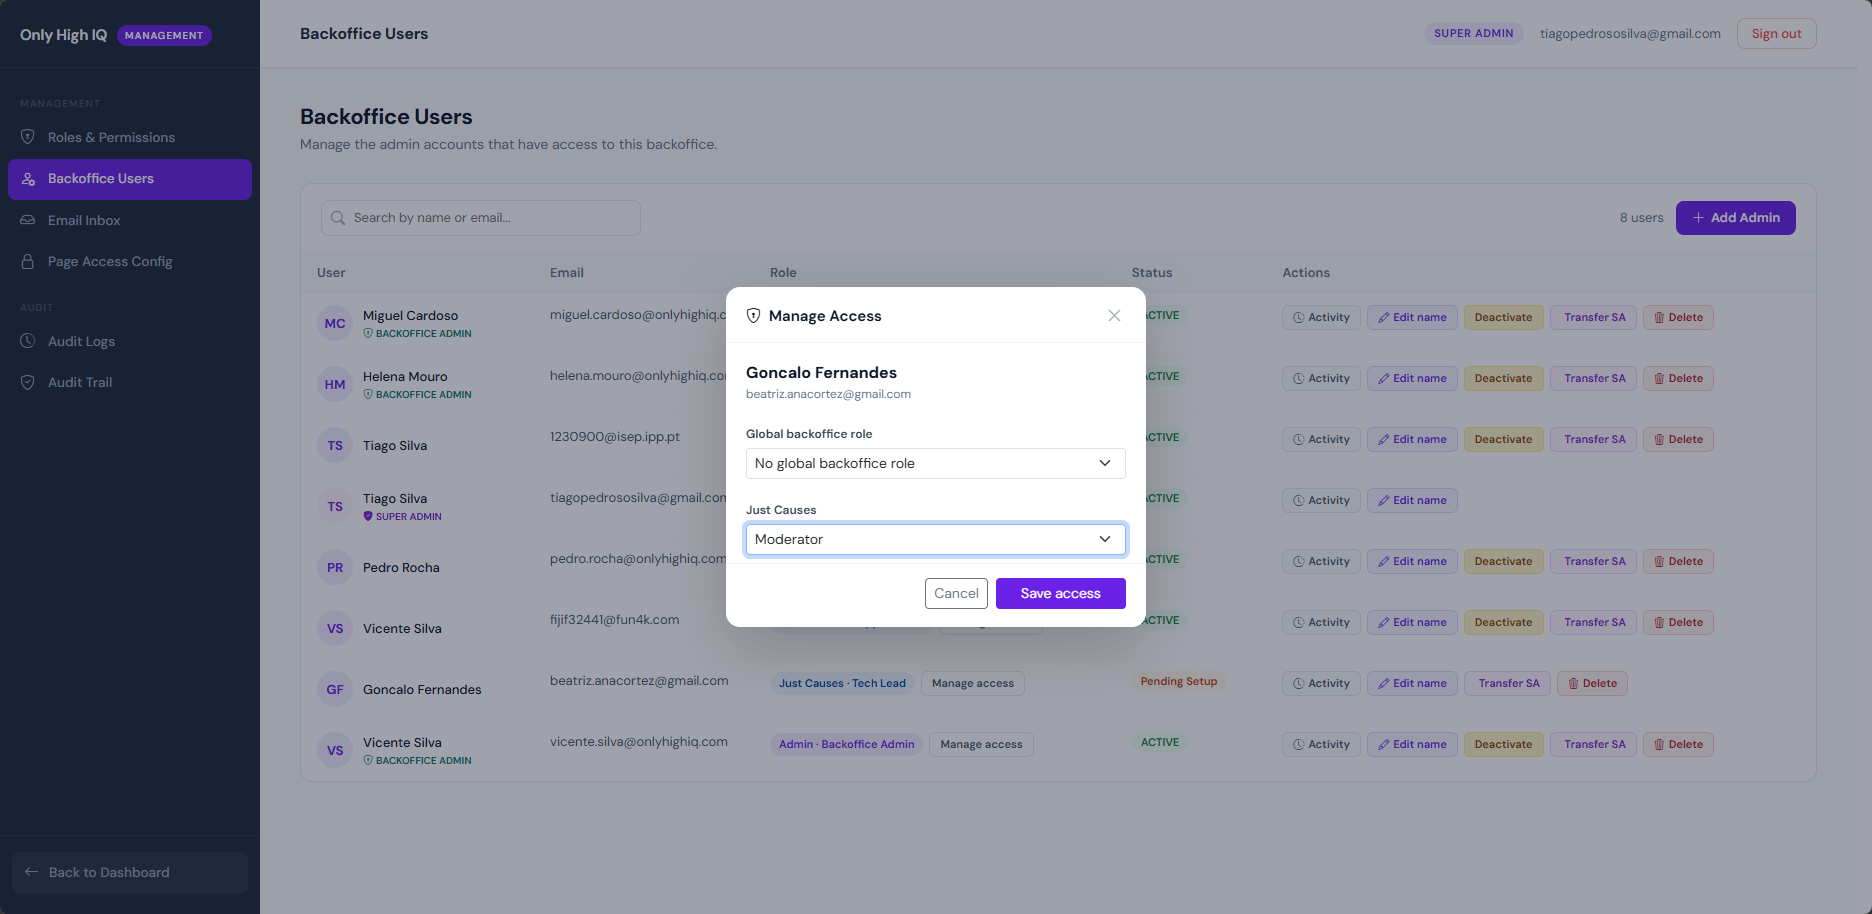
\includegraphics[width=0.95\textwidth, keepaspectratio]{frontmatter/assets/backoffice/ch4/role-assignment.png}
\caption{Atribuição de perfis a um operador interno}
\label{fig:impl_role_assignment}
\end{figure}

Depois da Figura~\ref{fig:impl_role_assignment}, a evidência a reter é que a atribuição de acesso é feita por aplicação. A janela distingue o perfil global de backoffice dos perfis da JustCauses e obriga o administrador a escolher explicitamente o acesso pretendido. Esta opção torna visível a regra usada no servidor: perfis administrativos são globais, enquanto perfis de aplicações operacionais são atribuídos no contexto da respetiva aplicação.
}{}

\IfFileExists{frontmatter/assets/backoffice/ch4/permissions-by-application.png}{
\begin{figure}[H]
\centering
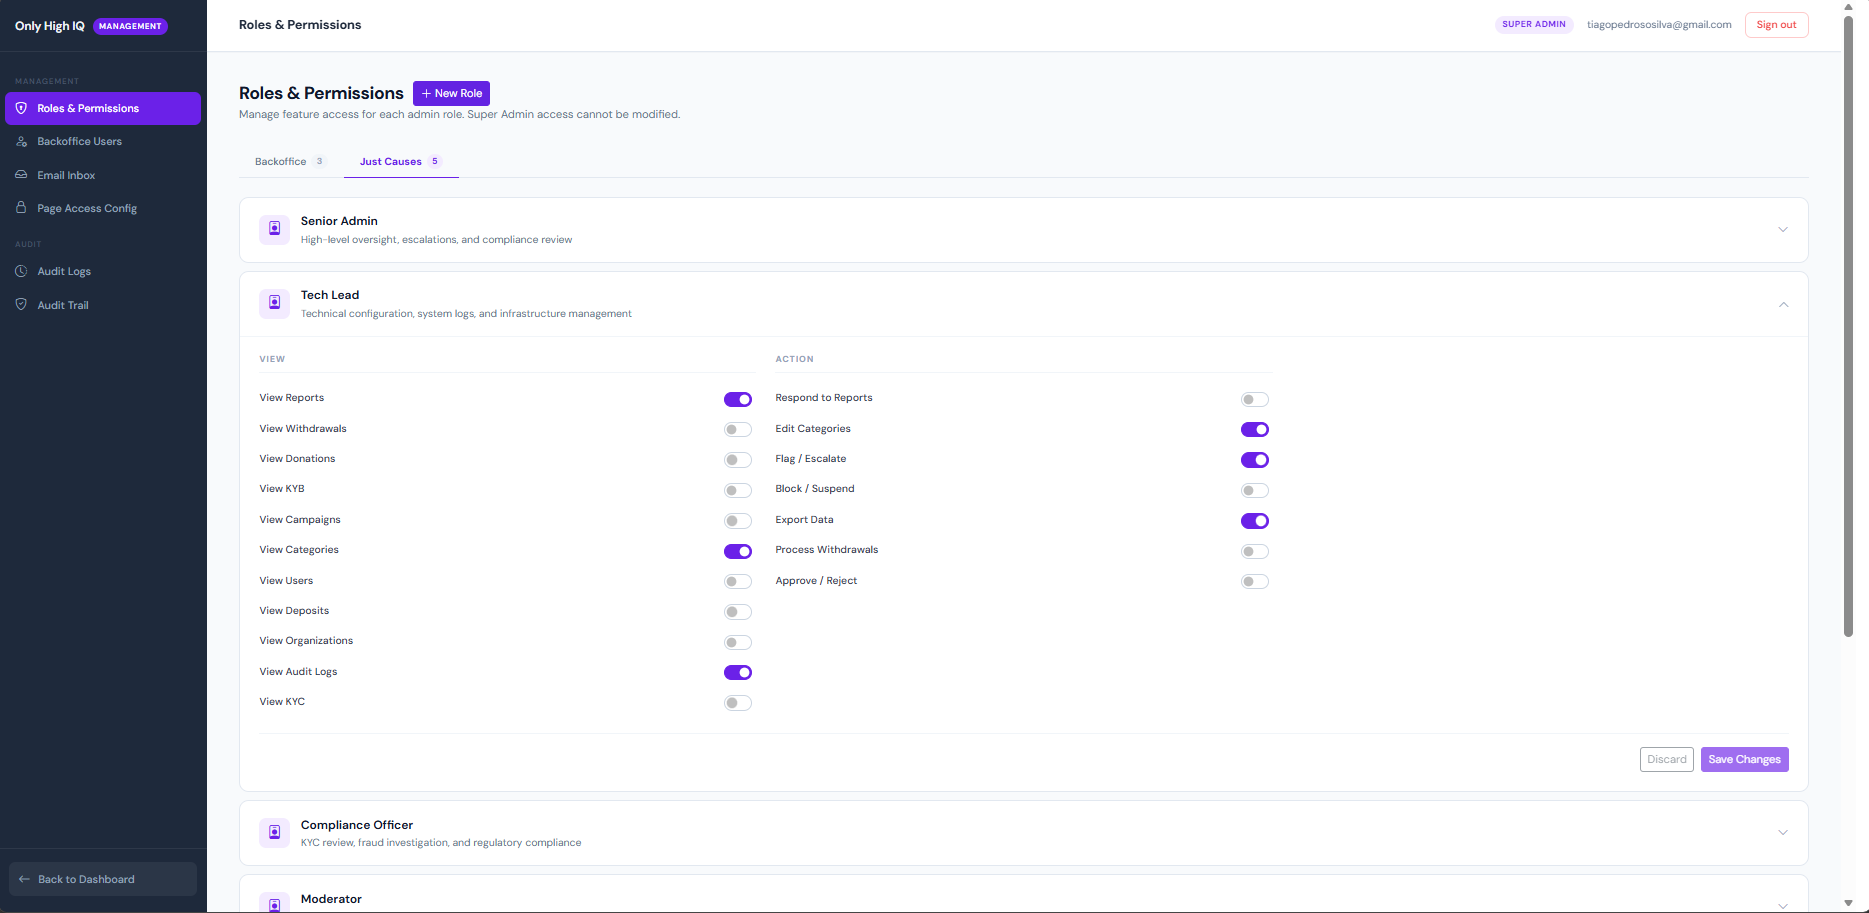
\includegraphics[width=0.95\textwidth, keepaspectratio]{frontmatter/assets/backoffice/ch4/permissions-by-application.png}
\caption{Permissões filtradas pela aplicação do perfil}
\label{fig:impl_permissions_by_application}
\end{figure}

Depois da Figura~\ref{fig:impl_permissions_by_application}, a evidência pretendida é a separação entre aplicações. O perfil aberto pertence à JustCauses e, por isso, a interface apresenta permissões ligadas a essa aplicação. A filtragem reduz erro operacional, mas não substitui a validação do servidor, que continua a rejeitar permissões cuja aplicação não corresponda à aplicação do perfil.
}{}

\IfFileExists{frontmatter/assets/backoffice/ch4/page-gates.png}{
\begin{figure}[H]
\centering
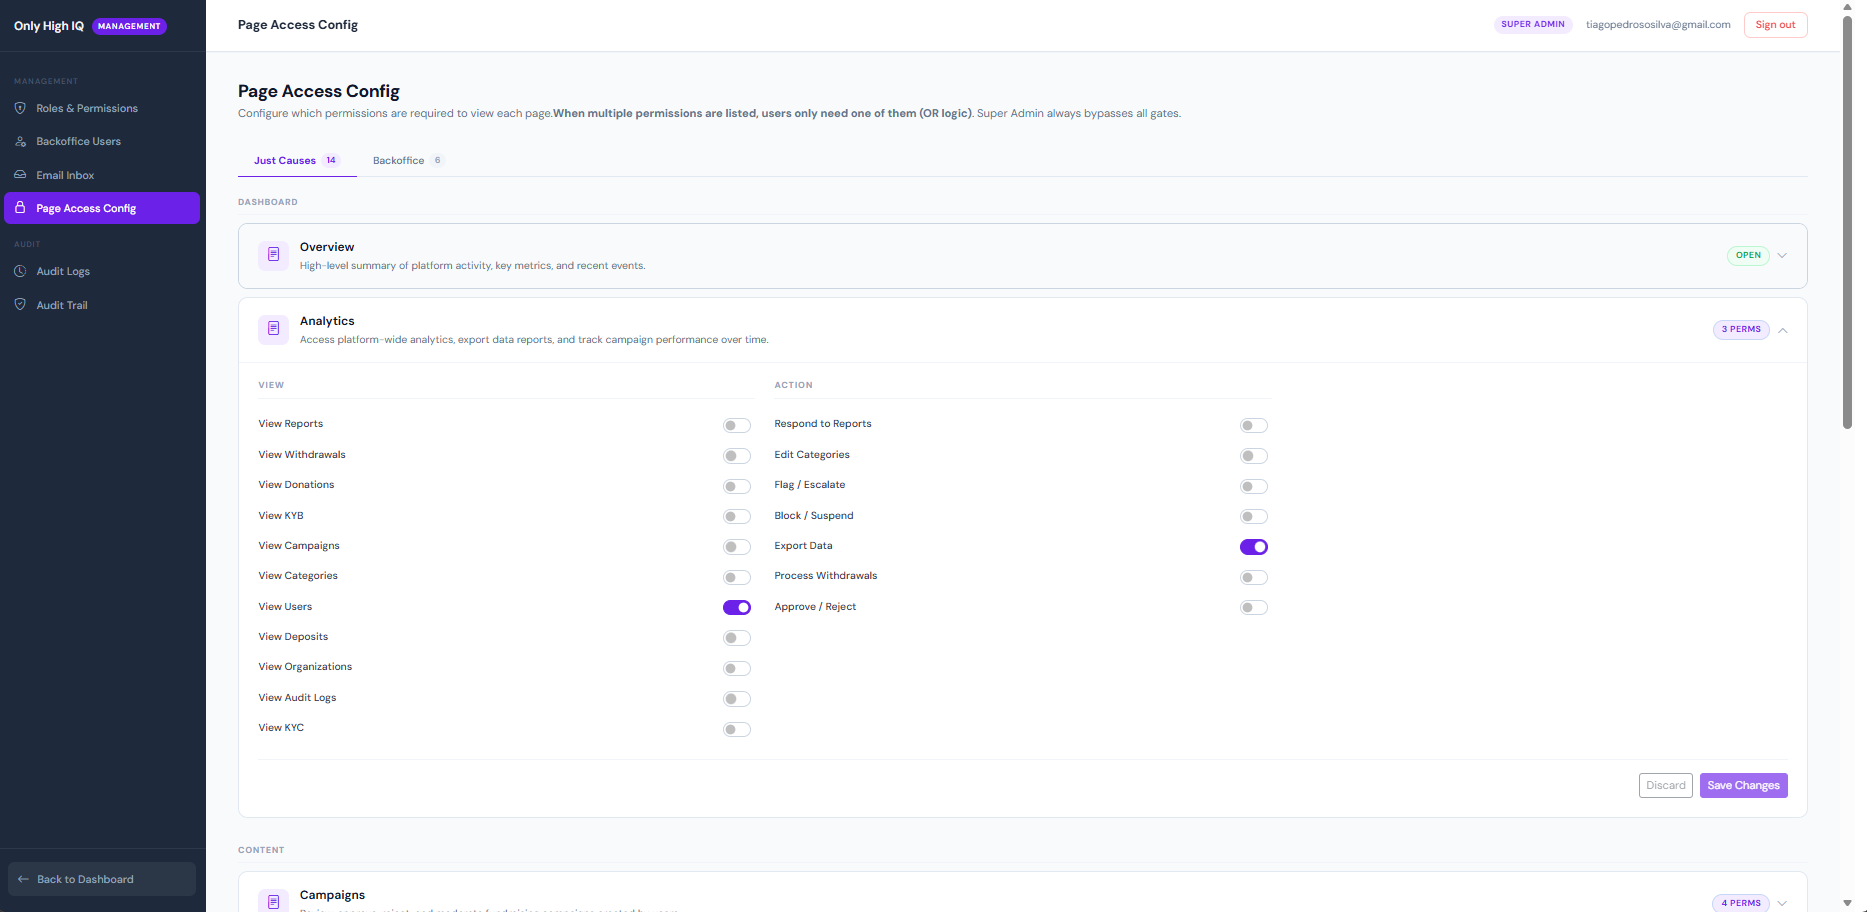
\includegraphics[width=0.95\textwidth, keepaspectratio]{frontmatter/assets/backoffice/ch4/page-gates.png}
\caption{Configuração administrativa dos \textit{page gates}}
\label{fig:impl_page_gates}
\end{figure}

Depois da Figura~\ref{fig:impl_page_gates}, importa evidenciar que o acesso a páginas não está fixo apenas no código. Cada página pode ter permissões associadas e a configuração é organizada por aplicação. No exemplo, a página de \textit{analytics} da JustCauses exige permissões específicas, enquanto páginas abertas aparecem explicitamente como \textit{open}. Esta distinção ajuda o administrador a perceber que páginas dependem de autorização e que páginas ficam disponíveis sem configuração adicional.
}{}

\IfFileExists{frontmatter/assets/backoffice/ch4/user-activity.png}{
\begin{figure}[H]
\centering
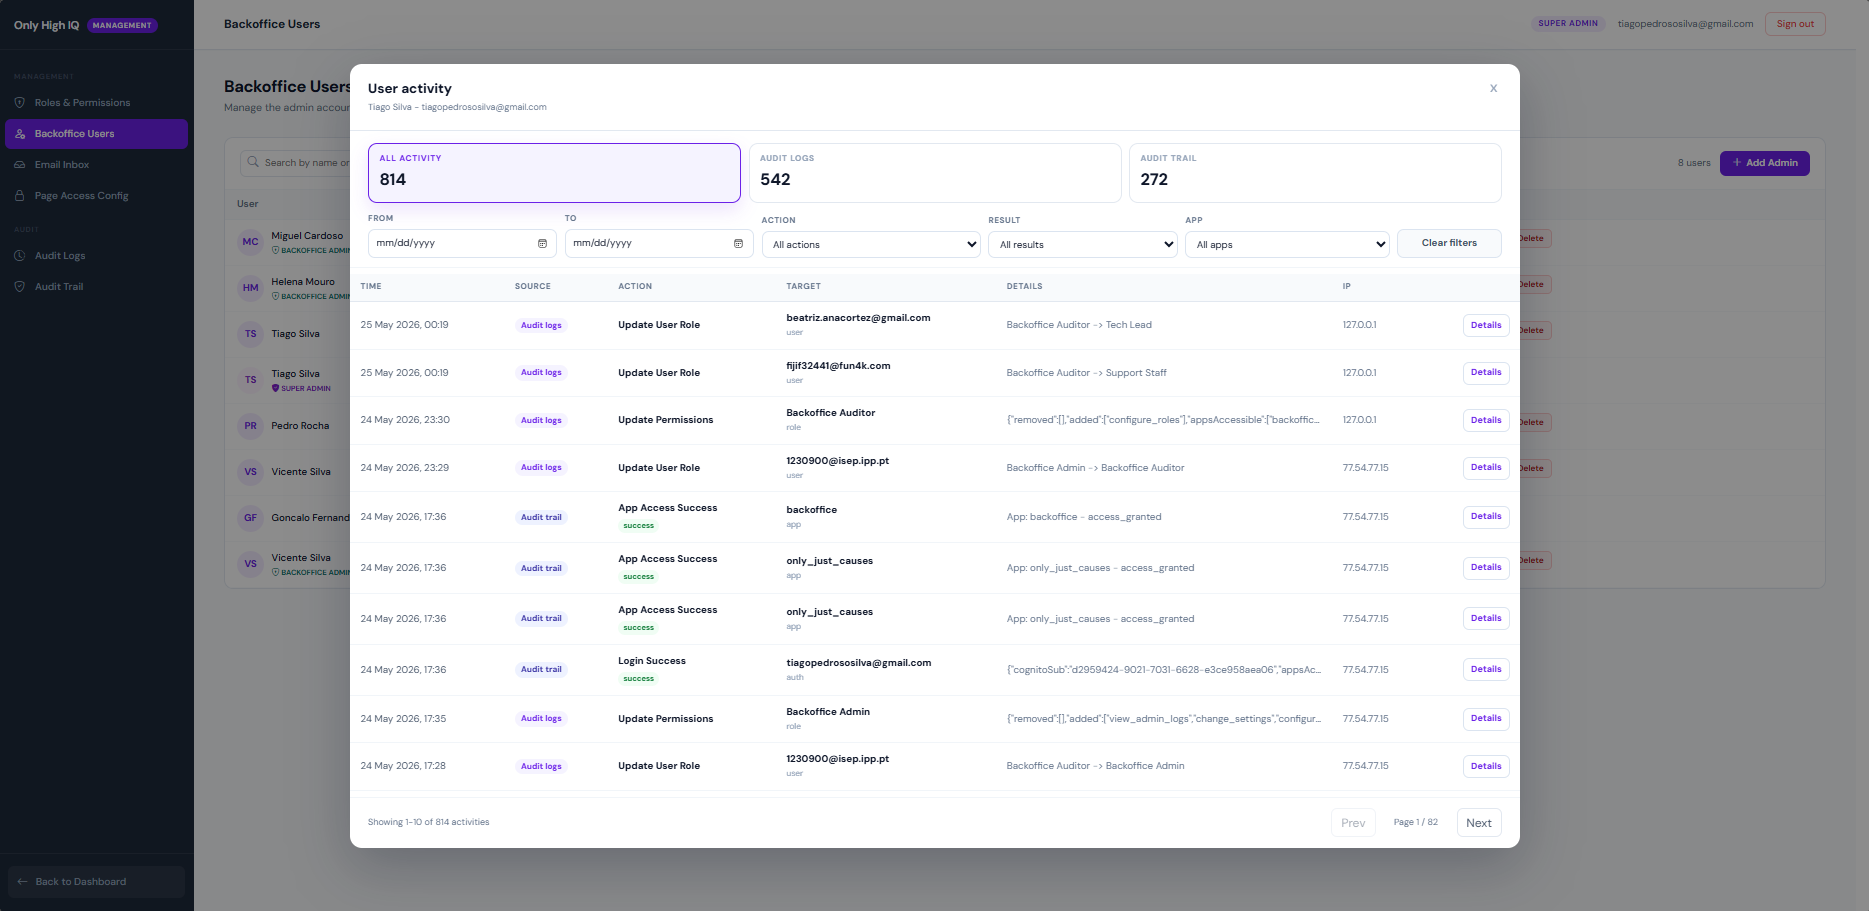
\includegraphics[width=0.95\textwidth, keepaspectratio]{frontmatter/assets/backoffice/ch4/user-activity.png}
\caption{Vista de atividade individual de um operador}
\label{fig:impl_user_activity}
\end{figure}

Depois da Figura~\ref{fig:impl_user_activity}, o objetivo é mostrar a dimensão de responsabilização. A vista agrega eventos de \textit{audit logs} e \textit{audit trail}, permite filtrar por ação, resultado e aplicação, e apresenta eventos como alterações de perfil, atualizações de permissões, acessos concedidos e início de sessão. Esta consulta apoia a análise do comportamento de um operador sem exigir navegação separada por vários registos.
}{}

\IfFileExists{frontmatter/assets/backoffice/ch4/ojc-campaign-review1.png}{
\begin{figure}[H]
\centering
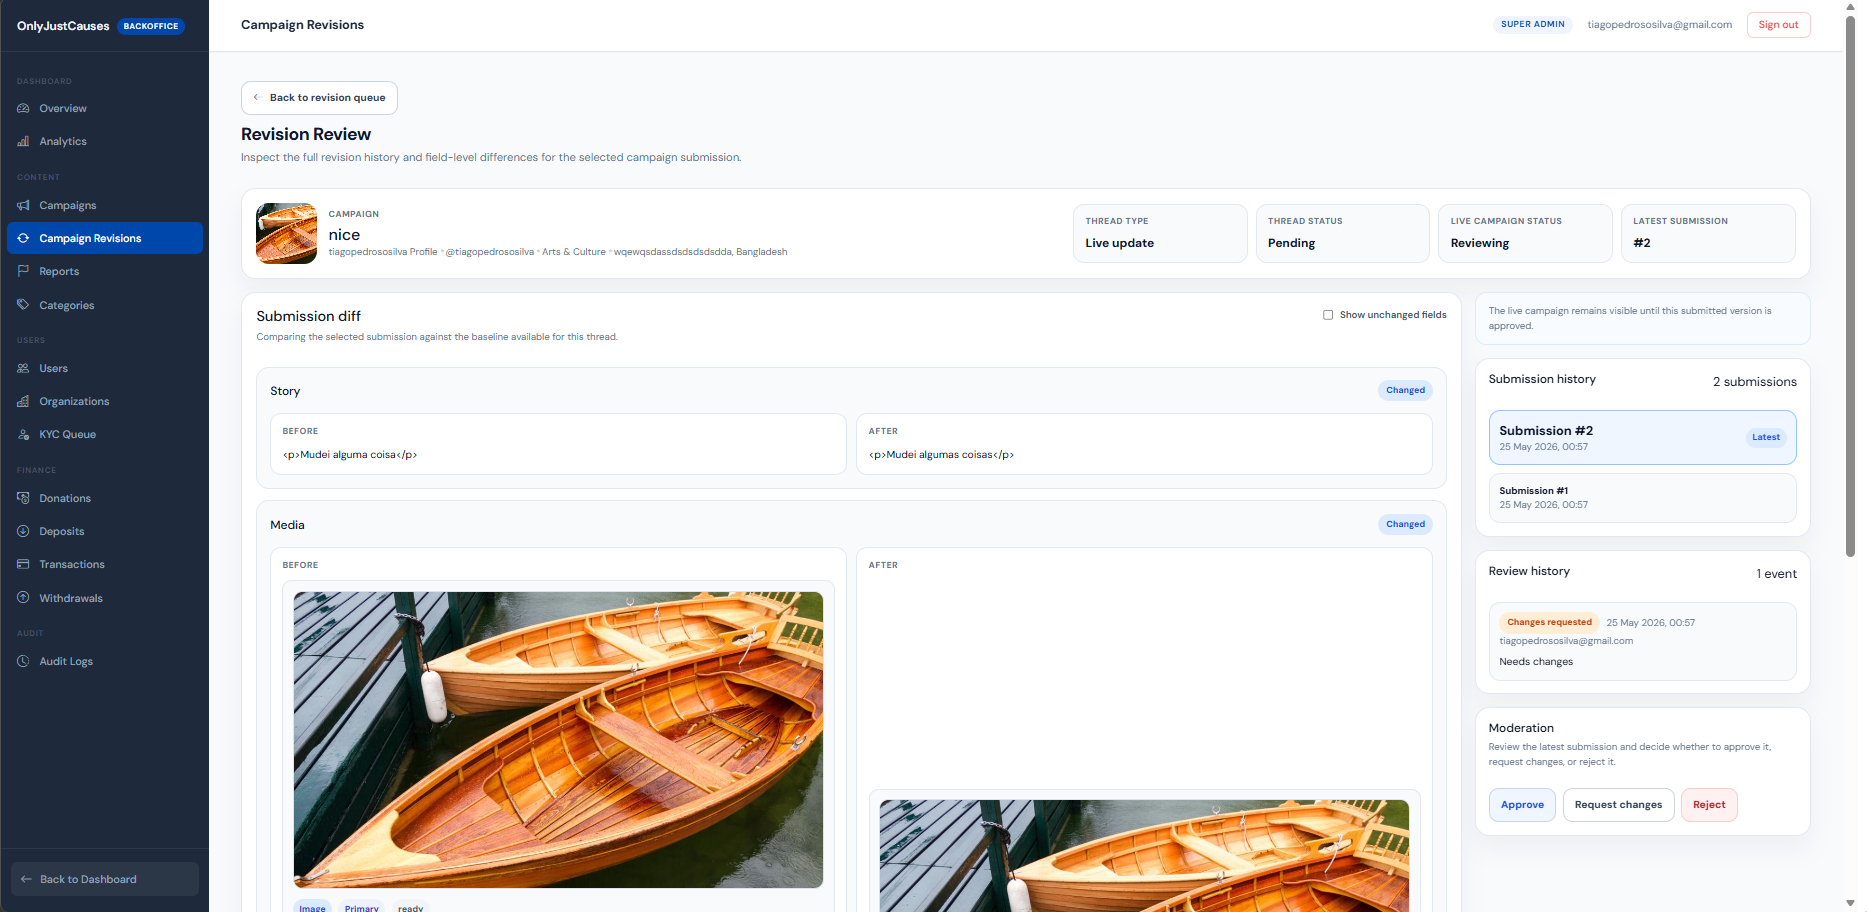
\includegraphics[width=0.95\textwidth, keepaspectratio]{frontmatter/assets/backoffice/ch4/ojc-campaign-review1.png}
\caption{Vista geral de uma \textit{thread} de revisão de campanha}
\label{fig:impl_ojc_campaign_review_thread}
\end{figure}

Depois da Figura~\ref{fig:impl_ojc_campaign_review_thread}, a evidência a reter é que a revisão de campanhas não consiste apenas em alterar um estado numa tabela. A vista reúne o resumo da campanha, o tipo e estado da \textit{thread}, a submissão selecionada, a comparação de conteúdo, o histórico de submissões, o histórico de decisões e as ações de moderação. O operador consegue assim decidir com contexto suficiente e a decisão fica associada à submissão que foi efetivamente analisada.
}{}

\IfFileExists{frontmatter/assets/backoffice/ch4/ojc-campaign-review2.png}{
\begin{figure}[H]
\centering
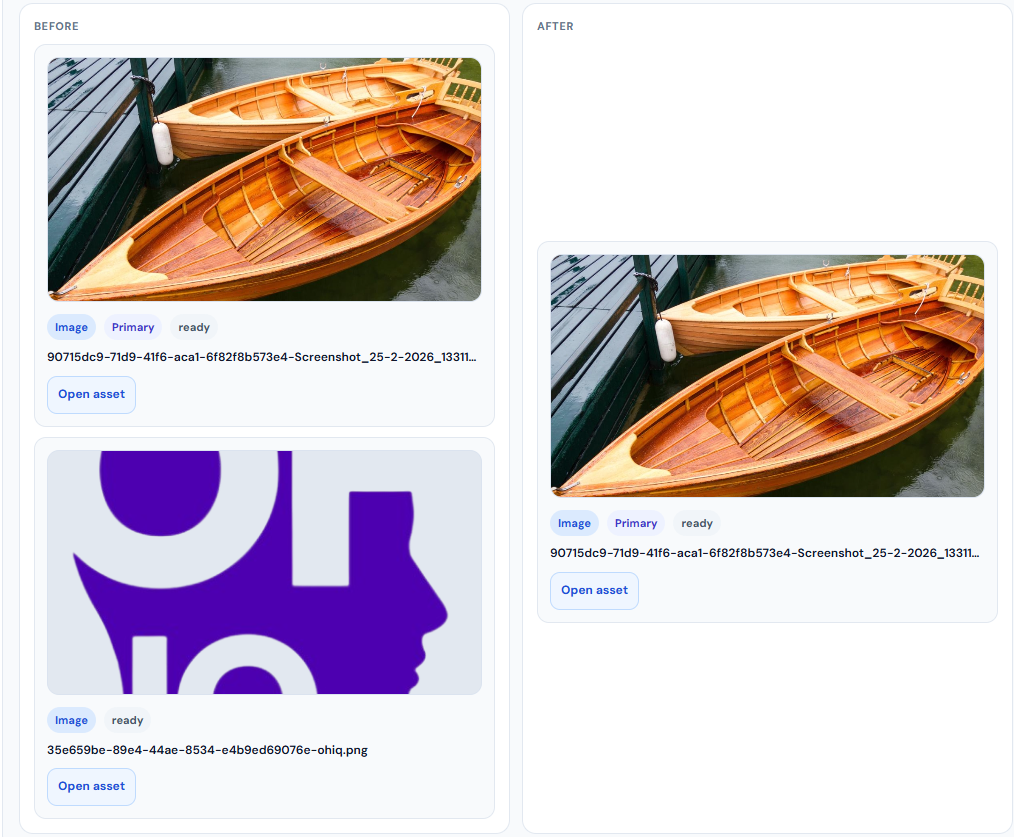
\includegraphics[width=0.82\textwidth, keepaspectratio]{frontmatter/assets/backoffice/ch4/ojc-campaign-review2.png}
\caption{Comparação de elementos multimédia numa revisão de campanha}
\label{fig:impl_ojc_campaign_review_media}
\end{figure}

Depois da Figura~\ref{fig:impl_ojc_campaign_review_media}, a leitura centra-se na comparação entre versões. O painel coloca lado a lado os elementos anteriores e os elementos submetidos, mantendo a indicação de ficheiro principal e o acesso direto ao recurso. Esta apresentação evita que a revisão de imagens dependa apenas da memória do operador ou de uma inspeção manual fora do backoffice.
}{}

\IfFileExists{frontmatter/assets/backoffice/ch4/campaign-review-modal-with-actions.png}{
\IfFileExists{frontmatter/assets/backoffice/ch4/campaign-review-modal-readonly.png}{
\begin{figure}[H]
\centering
\begin{minipage}[t]{0.49\textwidth}
\centering

\includegraphics[width=\linewidth, keepaspectratio]{frontmatter/assets/backoffice/ch4/campaign-review-modal-with-actions.png}
{\small Operador com permissões de ação}
\end{minipage}
\hfill
\begin{minipage}[t]{0.49\textwidth}
\centering

\includegraphics[width=\linewidth, keepaspectratio]{frontmatter/assets/backoffice/ch4/campaign-review-modal-readonly.png}
{\small Operador sem permissões de ação}
\end{minipage}
\caption{Comparação do modal de campanha com e sem permissões de ação}
\label{fig:impl_campaign_modal_permissions}
\end{figure}

Depois da Figura~\ref{fig:impl_campaign_modal_permissions}, a diferença relevante está nas ações disponíveis dentro do mesmo contexto funcional. Ambos os operadores conseguem consultar a campanha, mas apenas o operador com permissões adequadas vê os botões de intervenção, como \texttt{Deactivate}, \texttt{Finish}, \texttt{Request Changes} e \texttt{Campaign Revisions}. Esta evidência completa os exemplos anteriores de autorização: além do acesso à aplicação e à página, o backoffice também controla operações sensíveis dentro de um modal já aberto.
}{}}{}

\IfFileExists{frontmatter/assets/backoffice/ch4/transactional-email.png}{
\begin{figure}[H]
\centering
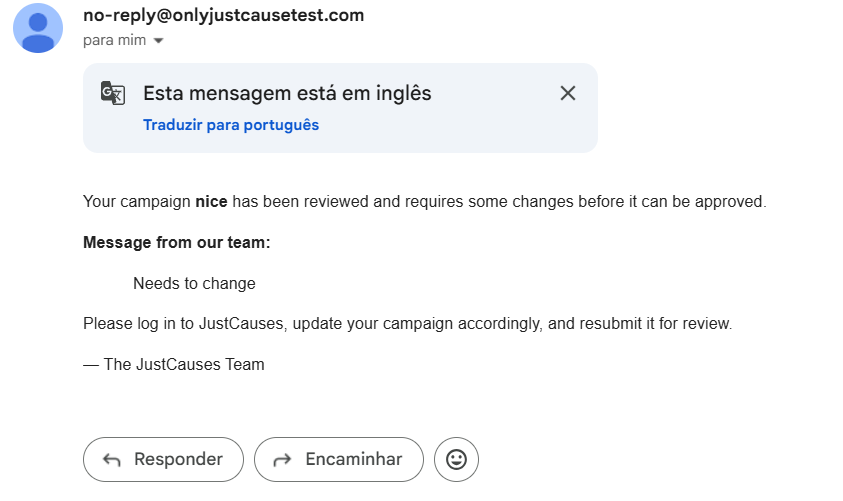
\includegraphics[width=0.82\textwidth, keepaspectratio]{frontmatter/assets/backoffice/ch4/transactional-email.png}
\caption{E-mail transacional enviado após pedido de alterações}
\label{fig:impl_transactional_email}
\end{figure}

Depois da Figura~\ref{fig:impl_transactional_email}, observa-se o resultado externo de uma decisão tomada no painel. A mensagem informa o criador de que a campanha precisa de alterações e inclui a nota definida pelo operador durante a revisão. Este exemplo liga três partes da implementação descritas neste capítulo: decisão administrativa, persistência da mensagem de revisão e envio automático por e-mail.
}{}

\IfFileExists{frontmatter/assets/backoffice/ch4/ojc-categories.png}{
\begin{figure}[H]
\centering
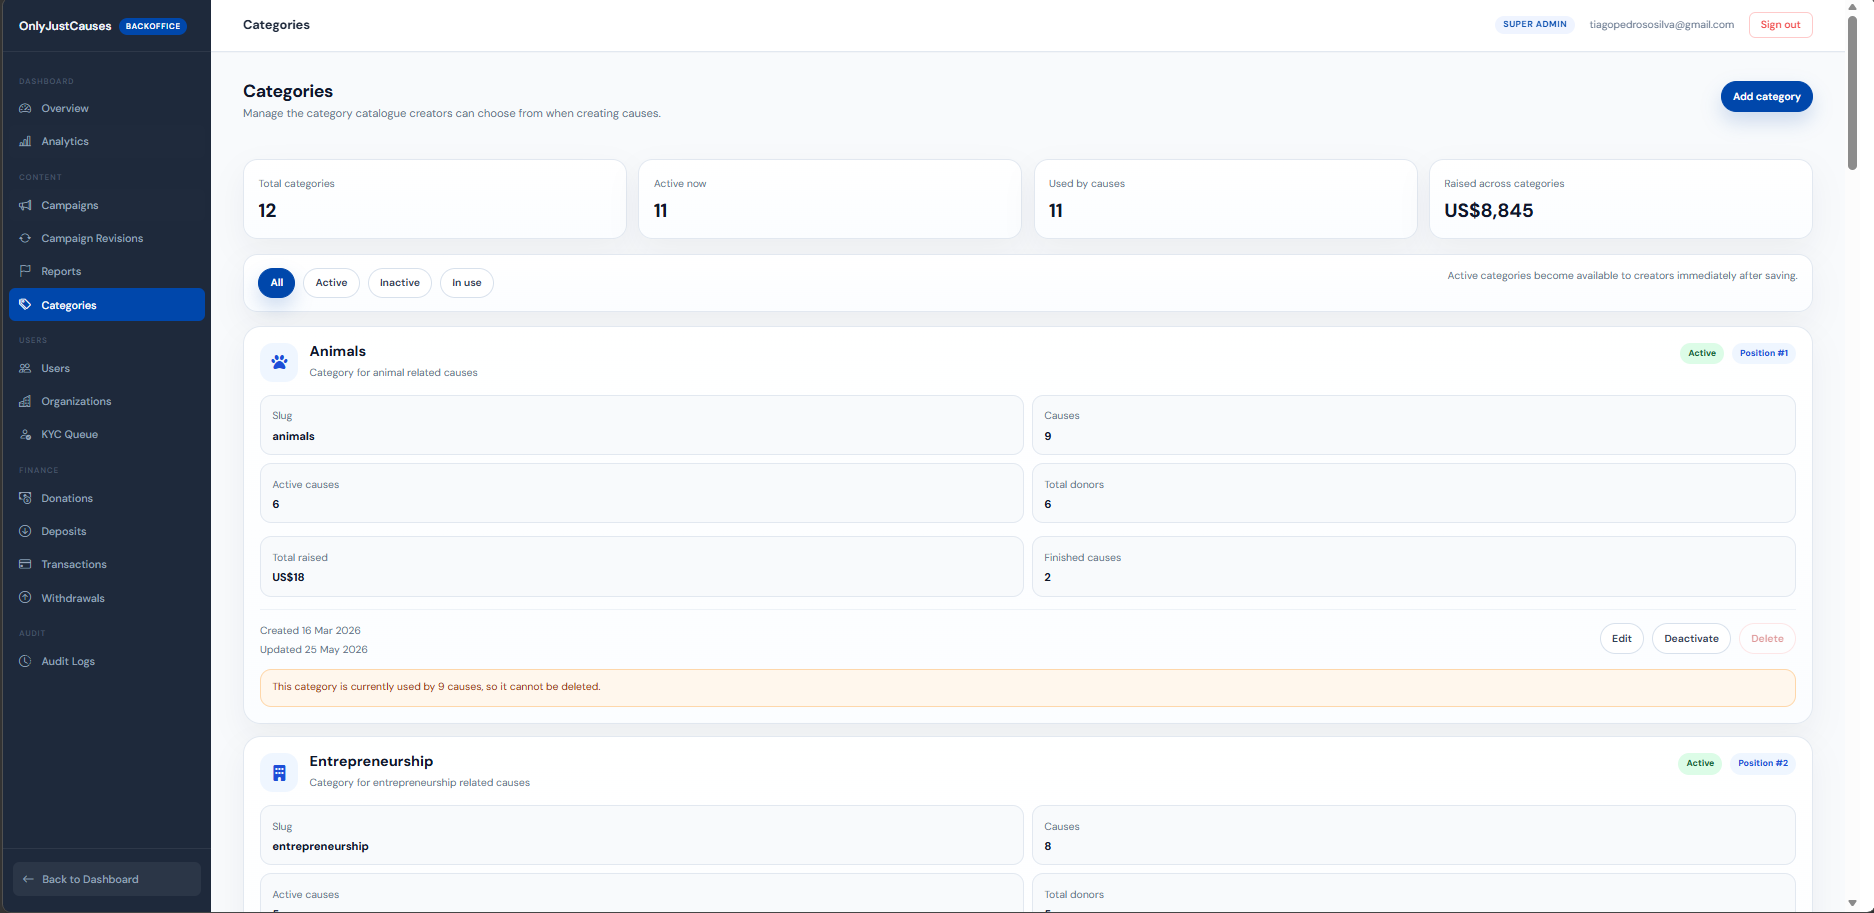
\includegraphics[width=0.95\textwidth, keepaspectratio]{frontmatter/assets/backoffice/ch4/ojc-categories.png}
\caption{Gestão de categorias da JustCauses}
\label{fig:impl_ojc_categories}
\end{figure}

Depois da Figura~\ref{fig:impl_ojc_categories}, a evidência a retirar é que a gestão de categorias não se limita a uma lista de nomes. A página mostra métricas agregadas, filtros por estado, posição de apresentação, número de causas associadas e ações permitidas. Quando uma categoria está em uso, a interface torna explícita a restrição de eliminação, evitando que o operador execute uma ação que afetaria campanhas existentes.
}{}

\IfFileExists{frontmatter/assets/backoffice/ch4/kyc-queue.png}{
\begin{figure}[H]
\centering
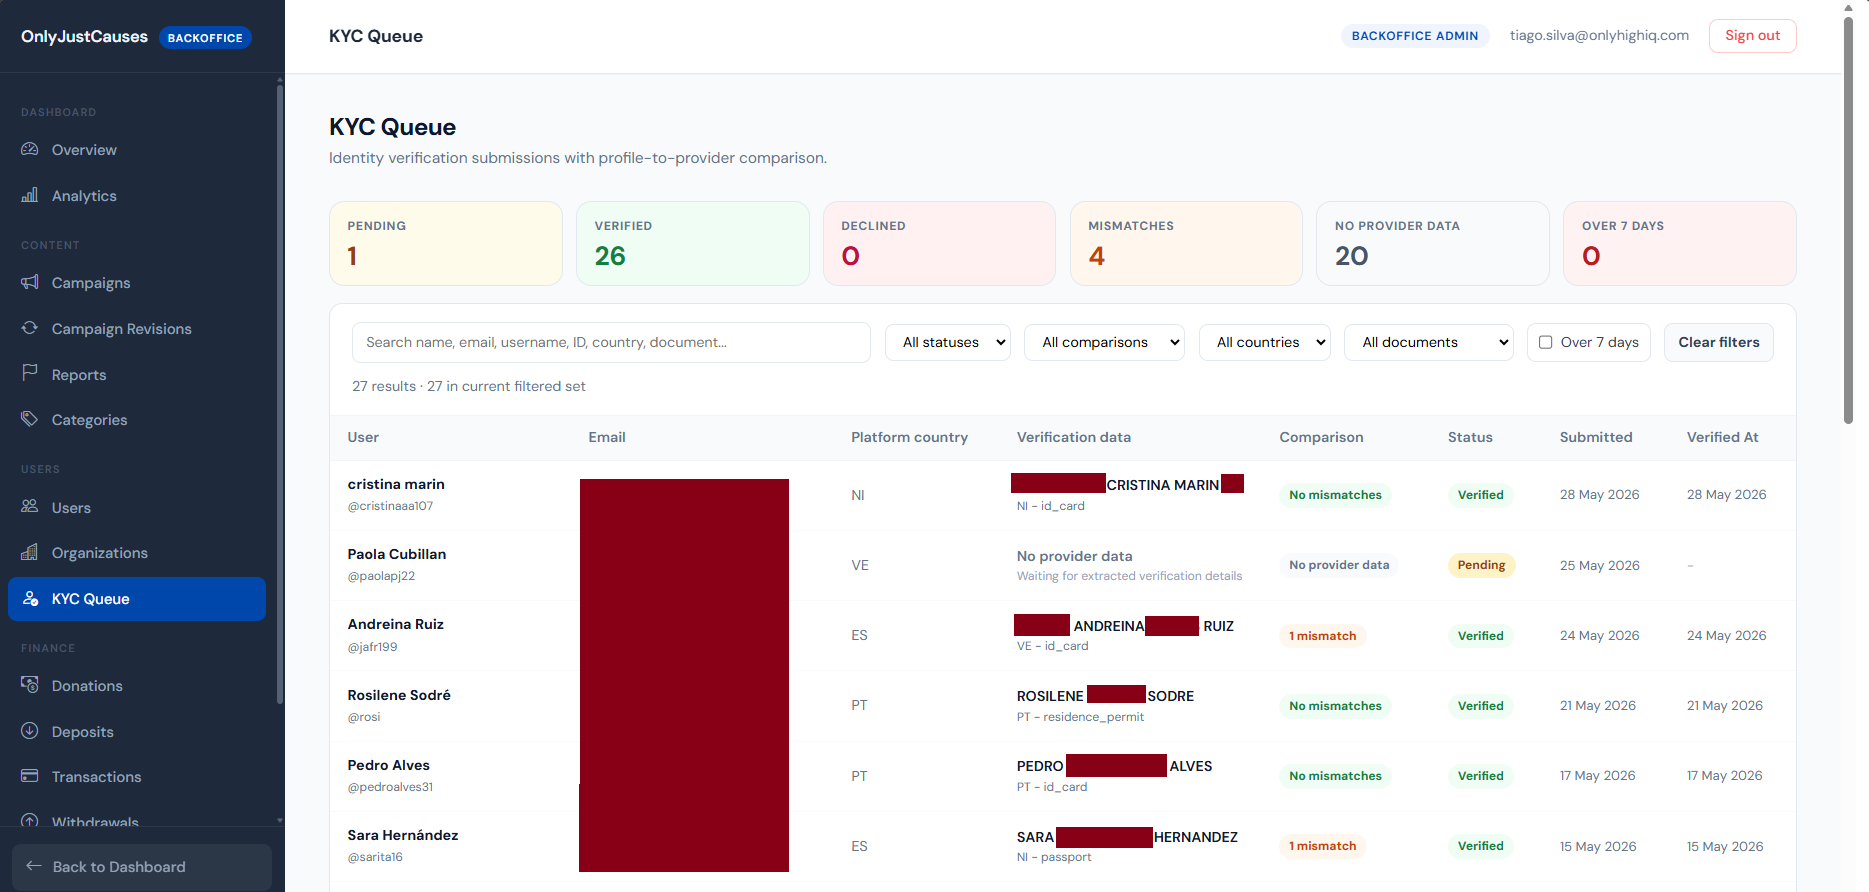
\includegraphics[width=0.95\textwidth, keepaspectratio]{frontmatter/assets/backoffice/ch4/kyc-queue.png}
\caption{Fila de verificação KYC de utilizadores individuais}
\label{fig:impl_kyc_queue}
\end{figure}

Depois da Figura~\ref{fig:impl_kyc_queue}, a evidência principal é a existência de uma fila operacional para acompanhar verificações de identidade. A página permite filtrar submissões por estado, comparação de dados, país, tipo de documento e atraso, mostrando ao operador quais os casos que exigem análise. Esta vista transforma dados provenientes do fornecedor de verificação e dos perfis da JustCauses numa lista acionável dentro do backoffice.
}{}

\IfFileExists{frontmatter/assets/backoffice/ch4/kyc-comparison-modal.png}{
\begin{figure}[H]
\centering
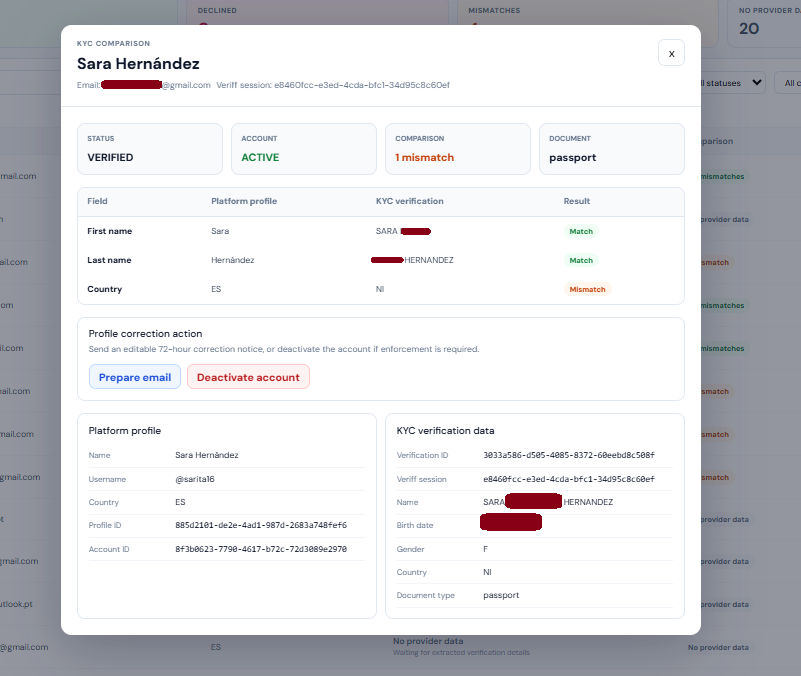
\includegraphics[width=0.78\textwidth, keepaspectratio]{frontmatter/assets/backoffice/ch4/kyc-comparison-modal.png}
\caption{Comparação entre perfil e dados de verificação KYC}
\label{fig:impl_kyc_comparison_modal}
\end{figure}

Depois da Figura~\ref{fig:impl_kyc_comparison_modal}, o ponto a reter é a comparação explícita entre a informação declarada pelo utilizador na plataforma e a informação devolvida pelo fornecedor de verificação. O operador não decide apenas com base no estado final da submissão: vê que campos coincidem, que campos divergem e que ação pode executar. Avisos ao utilizador, reinícios de submissões pendentes e alterações de estado ficam associados a auditoria.
}{}

\IfFileExists{frontmatter/assets/backoffice/ch4/kyb-organizations.png}{
\begin{figure}[H]
\centering
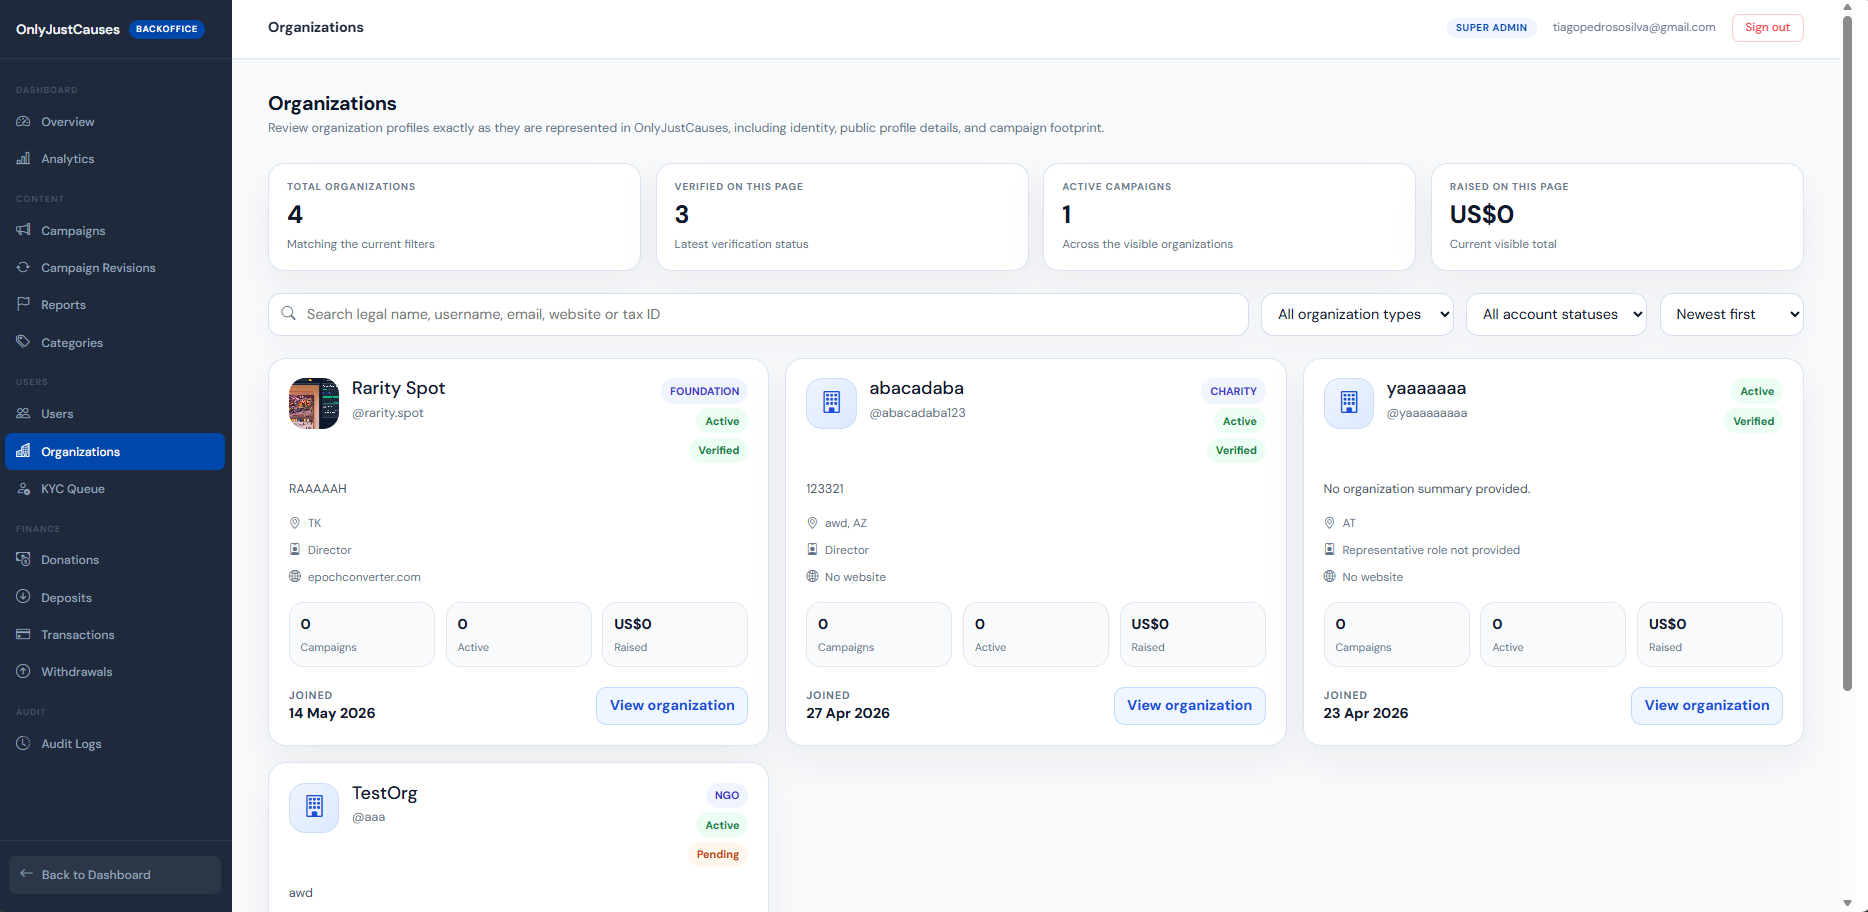
\includegraphics[width=0.95\textwidth, keepaspectratio]{frontmatter/assets/backoffice/ch4/kyb-organizations.png}
\caption{Organizações da JustCauses sujeitas a verificação KYB}
\label{fig:impl_kyb_organizations}
\end{figure}

Depois da Figura~\ref{fig:impl_kyb_organizations}, importa observar que as organizações são apresentadas como perfis coletivos do domínio da JustCauses. A listagem permite localizar entidades, consultar o seu estado operacional e perceber que organizações exigem análise documental. A figura prepara a leitura da verificação \gls{KYB}, sem transformar o módulo numa gestão genérica de organizações.
}{}

\IfFileExists{frontmatter/assets/backoffice/ch4/kyb-verification-modal.png}{
\begin{figure}[H]
\centering
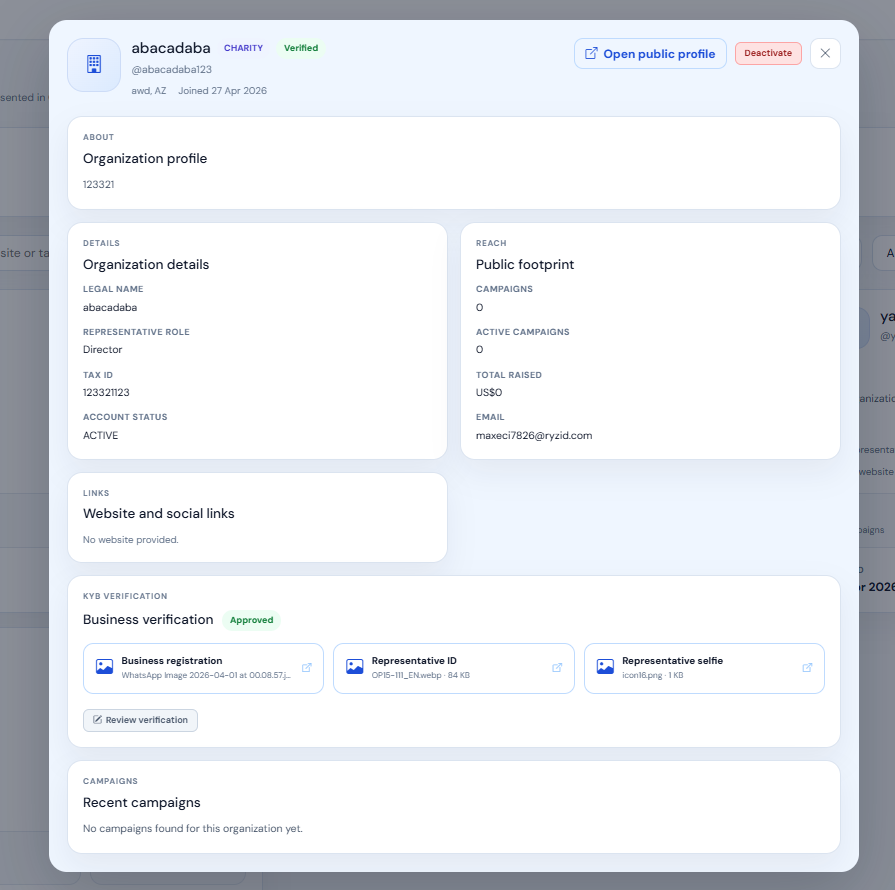
\includegraphics[width=0.72\textwidth, keepaspectratio]{frontmatter/assets/backoffice/ch4/kyb-verification-modal.png}
\caption{Submissão documental KYB de uma organização}
\label{fig:impl_kyb_verification_modal}
\end{figure}

Depois da Figura~\ref{fig:impl_kyb_verification_modal}, a evidência pretendida é a decisão administrativa sobre a oficialidade da organização. O operador consulta dados da entidade, documentos submetidos e estado da verificação antes de aprovar ou rejeitar a submissão. A decisão atualiza o estado de verificação da organização, gera notificação, pode enviar e-mail e fica registada em auditoria.
}{}

%----------------------------------------------------------------------------------------

\section{Testes}
\label{sec:testes}

A validação realizada no âmbito deste estágio combinou duas fontes principais de evidência: validação manual sistemática realizada durante o desenvolvimento e testes automatizados conduzidos pelo elemento da empresa responsável por \gls{QA}. Este relatório descreve a parte executada diretamente no desenvolvimento do backoffice, nomeadamente a utilização dos fluxos na aplicação, a confirmação dos estados apresentados na interface, a verificação das respostas da \gls{API} e a validação dos registos de auditoria gerados.

Os testes automatizados não foram desenvolvidos pelo autor deste relatório. Ainda assim, são relevantes para a avaliação da solução, porque incidem sobre endpoints, fluxos de interface e regras de autorização implementados neste projeto. Esta distinção mantém clara a autoria do trabalho e, ao mesmo tempo, enquadra a validação no processo real da empresa.

\subsection{Validação manual por módulo}
\label{subsec:testes_manual}

A validação manual consistiu em verificar cada módulo após a implementação. Para cada requisito funcional, foram executados cenários de sucesso, cenários de erro, ausência de permissões, persistência de dados e criação dos registos de auditoria esperados. Esta validação incidiu sobre os fluxos transversais de autenticação, autorização, gestão de perfis, \textit{page gates} e auditoria, bem como sobre os módulos da JustCauses. No final do processo, estes cenários foram considerados concluídos no âmbito definido para o estágio. A Tabela~\ref{tab:validacao_manual} resume os principais cenários verificados manualmente.

\begin{table}[H]
\caption{Cenários de validação manual da solução}
\label{tab:validacao_manual}
\begin{center}
\begingroup
\scriptsize
\setlength{\tabcolsep}{4pt}
\begin{tabular}{|>{\raggedright\arraybackslash}p{2.4cm}|>{\raggedright\arraybackslash}p{3.5cm}|>{\raggedright\arraybackslash}p{3.5cm}|>{\raggedright\arraybackslash}p{2.8cm}|}
\hline
\textbf{Módulo} & \textbf{Cenário validado} & \textbf{Resultado esperado} & \textbf{Evidência observada} \\ \hline
Autenticação & Operador inicia sessão com conta ativa & Sessão criada e contexto interno carregado & Redirecionamento para o seletor de aplicações \\ \hline
Acesso a aplicações & Operador sem acesso tenta abrir uma aplicação & Acesso recusado & Ecrã de acesso negado e registo de tentativa \\ \hline
Perfis por aplicação & Administrador atribui perfis a um operador & Só é aceite um perfil por aplicação; backoffice é exclusivo & Atualização persistida e refletida no perfil do utilizador \\ \hline
Permissões & Tentativa de associar permissão de outra aplicação a um perfil & Pedido rejeitado pelo servidor & Resposta de erro e ausência de alteração persistida \\ \hline
\textit{Page gates} & Operador sem permissão tenta aceder a página protegida & Página não é apresentada ou pedido é recusado & Navegação bloqueada e auditoria de recusa \\ \hline
Campanhas & Aprovar, rejeitar ou pedir alterações & Estado atualizado, mensagem registada e auditoria criada & Listagem atualizada e evento de auditoria persistido \\ \hline
Categorias & Criar ou editar categoria & Categoria persistida, duplicados rejeitados & Tabela atualizada ou erro de conflito \\ \hline
KYC/KYB & Rever uma verificação individual ou uma submissão documental de organização & Decisão aplicada, utilizador ou organização notificado e auditoria gerada & Estado de verificação atualizado e evento persistido \\ \hline
Atividade de utilizador & Abrir botão \textbf{Activity} num operador & Histórico filtrável por origem, ação, resultado e aplicação & Modal apresenta logs, audit trail e detalhes \\ \hline
\end{tabular}
\endgroup
\end{center}
\end{table}

Um dos cenários de validação manual incidiu sobre a tentativa de contornar a navegação normal do painel através da introdução direta de uma rota protegida no browser. A Figura~\ref{fig:test_access_denied_manual_route} apresenta esse comportamento para a rota \texttt{/ojc/analytics}, quando acedida por um operador que tem acesso à aplicação JustCauses, mas não tem permissão para essa página específica.

\IfFileExists{frontmatter/assets/backoffice/ch4/access-denied-manual-route.png}{
\begin{figure}[H]
\centering
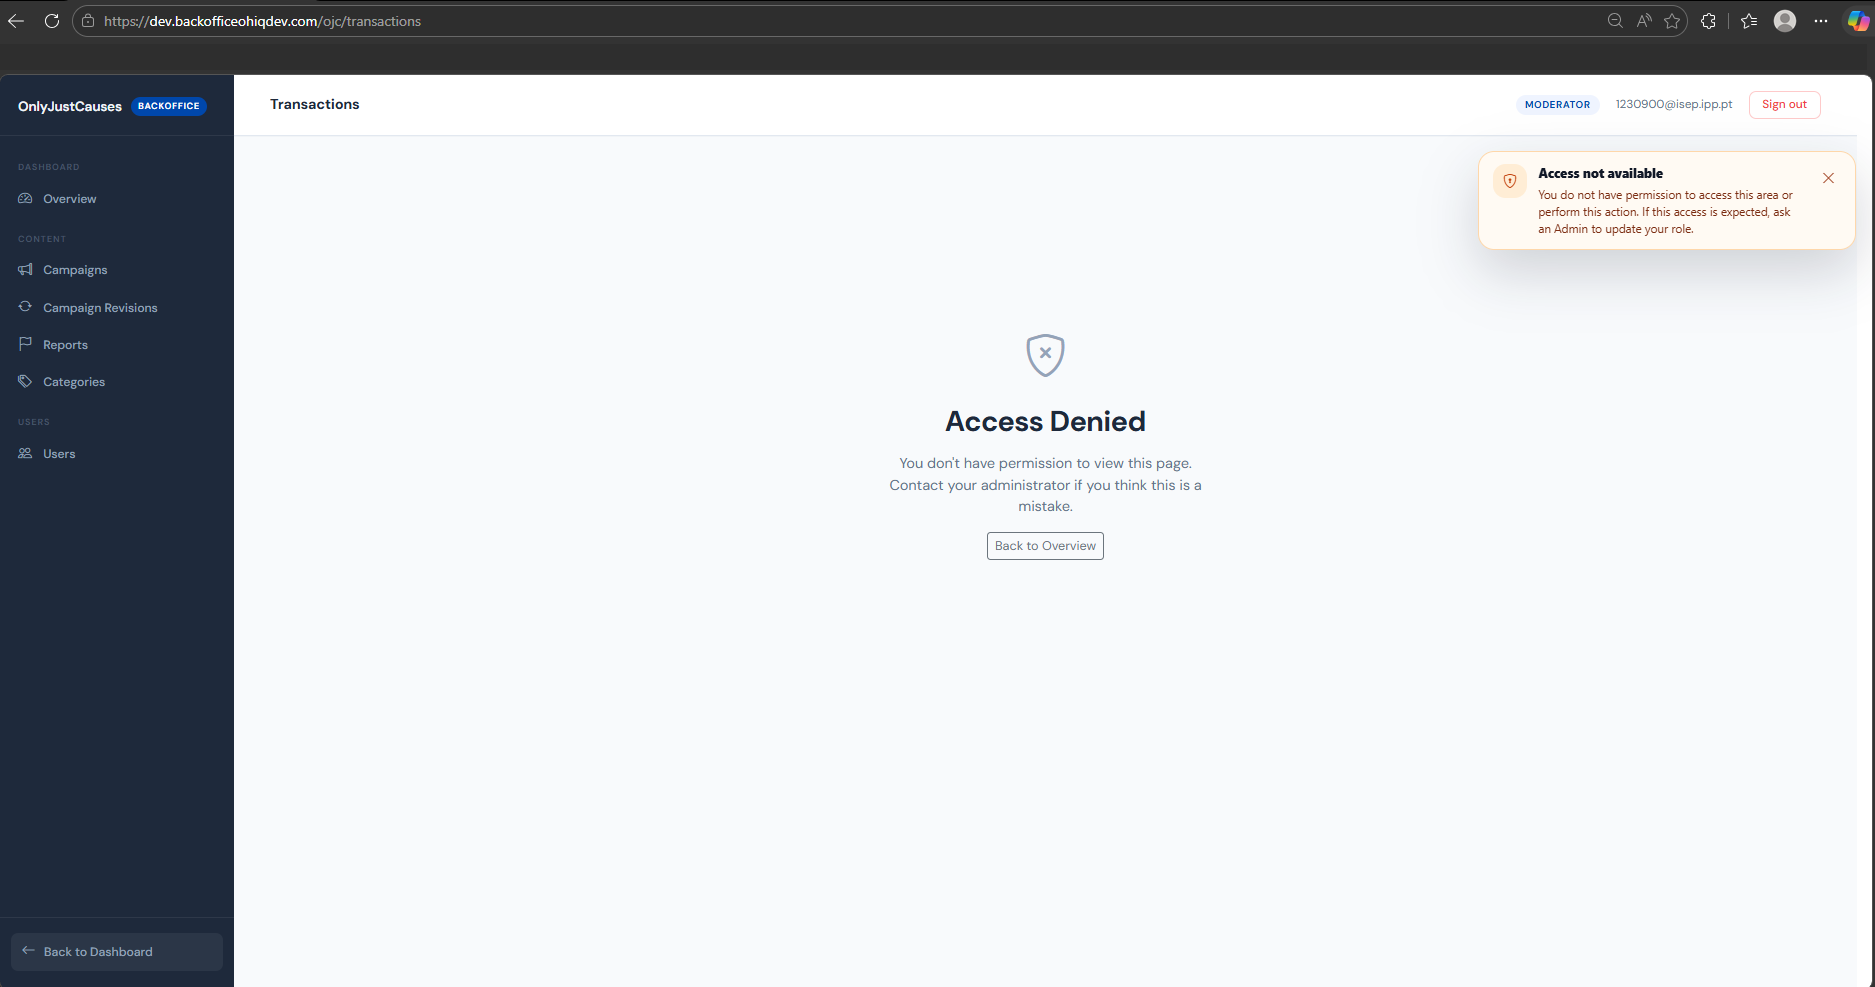
\includegraphics[width=0.95\textwidth, keepaspectratio]{frontmatter/assets/backoffice/ch4/access-denied-manual-route.png}
\caption{Validação manual de acesso negado a página protegida}
\label{fig:test_access_denied_manual_route}
\end{figure}

Depois da Figura~\ref{fig:test_access_denied_manual_route}, a evidência pretendida é que o controlo de acesso não se limita ao nível da aplicação. O operador consegue entrar no painel da JustCauses, mas não consegue abrir uma página para a qual o seu perfil não tem permissão. Mesmo quando a rota é introduzida manualmente, o \textit{page gate} bloqueia a navegação e apresenta um estado de acesso negado. No caso complementar, em que o operador não pertence sequer à aplicação, a validação ocorre antes da renderização do painel interno: é apresentada uma página completa de acesso negado, sem navegação lateral nem separadores da aplicação. Assim, a solução cobre tanto a entrada numa aplicação como o acesso a páginas específicas dentro dessa aplicação. As operações sensíveis continuam a ser verificadas no servidor através do \textit{middleware} de autorização.
}{}

Esta abordagem permitiu acompanhar o ritmo de desenvolvimento das \textit{sprints}, confirmar os fluxos antes da passagem das tarefas para concluído e identificar regressões visíveis durante a fase de testes iniciada a 13 de maio de 2026. A validação manual descrita neste relatório foi complementada pelos testes automatizados realizados pelo colega responsável por essa frente, pelo que a validação da solução ficou concluída dentro do processo de qualidade seguido pela empresa.

\subsection{Testes de código no processo de qualidade}
\label{subsec:testes_qa}

Na empresa, a criação e manutenção dos testes automatizados estava atribuída a um elemento específico da equipa. A sua existência foi importante durante o estágio, porque obrigou a estabilizar contratos de \gls{API}, códigos de resposta, identificadores de interface e estados de erro. Desta forma, as alterações feitas ao modelo de utilizadores, perfis, permissões, \textit{page gates} e auditoria puderam ser avaliadas não apenas por utilização manual, mas também contra cenários automatizados definidos pela equipa de qualidade.

Os artefactos disponíveis estão organizados em três conjuntos. O primeiro conjunto contém testes de \gls{API} em Playwright, focados em autenticação, utilizadores internos, perfis, permissões, \textit{page gates}, logs e estado do serviço. O segundo conjunto contém testes \gls{E2E} em Playwright, executados em browser, que validam fluxos de \textit{login}, \textit{dashboard}, navegação, gestão de utilizadores, auditoria, perfis e configuração de acessos. O terceiro conjunto contém testes de integração em Jest/Supertest, executáveis diretamente contra a \gls{API}, com cenários próximos dos testes de \gls{API}, mas estruturados ao nível de integração de endpoints. A Tabela~\ref{tab:testes_qa} caracteriza estes conjuntos de testes.

\begin{table}[H]
\caption{Caracterização dos testes automatizados de qualidade}
\label{tab:testes_qa}
\begin{center}
\begingroup
\scriptsize
\setlength{\tabcolsep}{4pt}
\begin{tabular}{|>{\raggedright\arraybackslash}p{2.5cm}|>{\raggedright\arraybackslash}p{4.2cm}|>{\raggedright\arraybackslash}p{1.5cm}|>{\raggedright\arraybackslash}p{4.5cm}|}
\hline
\textbf{Conjunto} & \textbf{Âmbito principal} & \textbf{Casos} & \textbf{Resultado ou observação} \\ \hline
\gls{API} Playwright & Autenticação, utilizadores, perfis, permissões, \textit{page gates}, logs e estado do serviço & 223 & Executados no relatório de 27/05/2026, sem falhas, erros ou testes ignorados \\ \hline
\gls{E2E} Playwright & \textit{Login}, \textit{dashboard}, navegação, gestão de operadores, auditoria, perfis e configuração de páginas & 96 & Executados no mesmo relatório, também sem falhas, erros ou testes ignorados \\ \hline
Integração Jest/Supertest & Validação direta de endpoints e contratos da \gls{API} em cenários de integração & 127 & Casos definidos para execução separada, cobrindo os mesmos módulos transversais de administração \\ \hline
\textbf{Total Playwright executado} & \textbf{API + E2E} & \textbf{319} & \textbf{319 testes concluídos com sucesso em 134,6 s, com 0 falhas, 0 erros e 0 ignorados} \\ \hline
\textbf{Total identificado} & \textbf{Playwright + integração} & \textbf{446} & \textbf{Cobertura funcional centrada nos módulos de autenticação, autorização, administração e auditoria} \\ \hline
\end{tabular}
\endgroup
\end{center}
\end{table}

A Listagem~\ref{lst:qa_page_gate_tests} apresenta um excerto representativo dos testes automatizados de \gls{API} sobre a configuração de acesso por página. O exemplo foi escolhido por incidir diretamente sobre uma regra central da solução: os \textit{page gates} pertencem a uma aplicação e a alteração das permissões exigidas deve ficar persistida no servidor. Por concisão, a listagem omite o carregamento inicial do identificador da página e da configuração original, realizado na preparação do teste.

\begin{lstlisting}[caption={Excerto de testes automatizados sobre configuração de acesso por página}, label={lst:qa_page_gate_tests}]
test('deve filtrar por application=just_causes', async ({ request }) => {
  const response =
    await request.get('/api/page-gates?application=just_causes');

  expect(response.status()).toBe(200);
  const gates = await response.json();
  expect(Array.isArray(gates)).toBe(true);

  for (const gate of gates) {
    expect(gate.application).toBe('just_causes');
  }
});

test('a atualizacao deve refletir no GET seguinte', async ({ request }) => {
  if (!gateId) return;
  const newPermissions: string[] = [];

  try {
    await request.put(`/api/page-gates/${gateId}`, {
      data: { requiredPermissions: newPermissions },
    });

    const getResponse =
      await request.get('/api/page-gates?application=just_causes');
    const gates = await getResponse.json();
    const updated = gates.find((g: any) => g.gateId === gateId);

    expect(updated).toBeDefined();
    expect(updated.requiredPermissions).toEqual(newPermissions);
  } finally {
    await request.put(`/api/page-gates/${gateId}`, {
      data: { requiredPermissions: originalPermissions },
    });
  }
});
\end{lstlisting}

O primeiro teste da Listagem~\ref{lst:qa_page_gate_tests} confirma que o filtro por aplicação não devolve configurações de outro domínio. O segundo altera temporariamente as permissões exigidas por uma página, valida a persistência através de uma nova leitura e repõe a configuração original no bloco \texttt{finally}. Este detalhe é relevante num ambiente partilhado, porque permite testar persistência real sem deixar dados artificiais na configuração do backoffice.

O relatório de execução Playwright consultado registou 319 testes concluídos com sucesso, sem falhas, erros, testes ignorados ou testes instáveis. Este resultado cobre os testes de \gls{API} e os testes \gls{E2E}. Os testes de integração em Jest/Supertest constam do conjunto de testes disponível e acrescentam 127 cenários definidos, mas não estavam incluídos no relatório Playwright, por serem executados através de um comando próprio.

Não foi disponibilizado um relatório de cobertura de código por linhas ou instruções. Por esse motivo, a avaliação quantitativa apresentada não deve ser lida como uma percentagem formal de cobertura. O que pode ser concluído com rigor é que existe cobertura funcional automatizada sobre os módulos mais sensíveis do backoffice: autenticação, resolução de utilizador autenticado, criação e manutenção de operadores, perfis, permissões, configuração de páginas, logs, audit trail e navegação administrativa.

Estes testes influenciaram o desenvolvimento de forma concreta. A implementação teve de manter contratos de \gls{API} estáveis, códigos de resposta previsíveis, validações explícitas, estados de erro distinguíveis e identificadores de interface adequados para automação. Isto foi particularmente relevante nas alterações ao modelo de perfis por aplicação e permissões por aplicação, porque os testes obrigam a que a interface, os endpoints e os dados devolvidos continuem alinhados após cada alteração.

%----------------------------------------------------------------------------------------

\section{Avaliação da solução}
\label{sec:avaliacao}

Para além dos testes, a solução foi avaliada pela sua adequação ao problema inicial: permitir operação interna da JustCauses e, simultaneamente, manter uma base técnica reutilizável para futuras aplicações. A disponibilização do backoffice em ambiente de utilização interna permitiu validar a viabilidade operacional dos fluxos principais, sobretudo nos módulos de autenticação, controlo de acesso, auditoria, revisão de campanhas e gestão de categorias.

\subsection{Avaliação operacional e critérios complementares}
\label{subsec:avaliacao_complementar}

A Tabela~\ref{tab:avaliacao_complementar} apresenta os critérios usados para complementar a validação funcional e automatizada.

\begin{table}[H]
\caption{Critérios complementares de avaliação da solução}
\label{tab:avaliacao_complementar}
\begin{center}
\begingroup
\scriptsize
\setlength{\tabcolsep}{4pt}
\begin{tabular}{|>{\raggedright\arraybackslash}p{2.4cm}|>{\raggedright\arraybackslash}p{5.2cm}|>{\raggedright\arraybackslash}p{4.5cm}|}
\hline
\textbf{Critério} & \textbf{Forma de avaliação} & \textbf{Resultado observado} \\ \hline
Adequação funcional & Comparação entre problema inicial, requisitos e funcionalidades implementadas & Os módulos prioritários da JustCauses e os mecanismos transversais de administração ficaram disponíveis no âmbito definido \\ \hline
Segurança e autorização & Validação manual e testes de \gls{API} sobre autenticação, permissões, perfis e acessos negados & A decisão de acesso é aplicada no cliente e revalidada no servidor, com registo auditável das recusas relevantes \\ \hline
Escalabilidade funcional & Verificação do modelo de aplicações, perfis por aplicação, permissões por aplicação e \textit{page gates} & A arquitetura suporta novas aplicações sem duplicar autenticação, autorização e auditoria \\ \hline
Qualidade automatizada & Relatório Playwright e testes de integração disponíveis no processo de \gls{QA} & 319 testes Playwright concluídos com sucesso e 127 testes de integração definidos sobre os módulos transversais \\ \hline
Usabilidade operacional & Utilização interna dos fluxos e revisão dos estados visíveis na interface & As páginas apresentam ações, filtros, estados de erro e mensagens explícitas para apoiar trabalho administrativo diário \\ \hline
Desempenho percebido & Utilização manual dos fluxos principais em ambiente de desenvolvimento e produção interna & Não foram identificados bloqueios funcionais nos fluxos avaliados, embora não tenha sido realizada uma medição formal de carga \\ \hline
Acessibilidade & Revisão visual e funcional dos componentes usados nas páginas principais & Foram mantidos padrões consistentes de navegação e contraste, mas não foi realizada uma auditoria automática formal de acessibilidade \\ \hline
\end{tabular}
\endgroup
\end{center}
\end{table}

Esta avaliação mostra que a solução responde ao núcleo do problema apresentado na introdução: reduzir operações manuais pouco rastreáveis, centralizar a administração da JustCauses e criar uma base de controlo de acesso reutilizável. Ao mesmo tempo, identifica limites da avaliação realizada. Não houve, até ao momento descrito neste relatório, um inquérito formal aos operadores internos nem uma campanha dedicada de testes de carga ou acessibilidade. A avaliação de usabilidade baseou-se, por isso, na utilização operacional e na revisão dos fluxos entregues. Esses instrumentos poderiam complementar a avaliação em iterações futuras, sobretudo quando o número de operadores e aplicações integradas aumentar.

\subsection{Estado final da solução}
\label{subsec:estado_final_solucao}

Esta secção avalia o estado de implementação da solução por eixo funcional, com base no estado do painel no final do período de desenvolvimento coberto por este relatório e nas evidências apresentadas nas secções anteriores. Em vez de voltar a detalhar cada fluxo operacional isolado, a análise centra-se nas capacidades que melhor representam o trabalho efetivamente consolidado e a sua correspondência com os objetivos definidos na introdução. A Tabela~\ref{tab:avaliacao_rf} sintetiza esse estado final.

\begin{table}[H]
\caption{Estado de implementação por eixo funcional}
\label{tab:avaliacao_rf}
\begin{center}
\begingroup
\scriptsize
\setlength{\tabcolsep}{4pt}
\begin{tabular}{|>{\raggedright\arraybackslash}p{2.3cm}|>{\raggedright\arraybackslash}p{3.2cm}|>{\raggedright\arraybackslash}p{1.2cm}|>{\raggedright\arraybackslash}p{1.8cm}|>{\raggedright\arraybackslash}p{3.7cm}|}
\hline
\textbf{Eixo} & \textbf{Descrição resumida} & \textbf{Estado} & \textbf{Obj.} & \textbf{Observações} \\ \hline
Autenticação com Cognito & Gestão de sessão, recuperação de palavra-passe e integração com o painel & Concluído & OE1.1 & Fluxo funcional com Amplify no cliente e validação JWT no servidor \\ \hline
Resolução do contexto de autorização & Perfis, aplicações acessíveis e permissões efetivas do operador & Concluído & OE1.1/OE1.2 & \texttt{/users/me} no cliente e \texttt{req.auth} no servidor mantêm a mesma fonte de verdade \\ \hline
Acesso a aplicações e páginas & Guardas de rota, redireções e \textit{page gates} por aplicação & Concluído & OE1.3/OE2.1 & Separação entre \texttt{backoffice} e \texttt{just\_causes}, com suporte a expansão para novas aplicações \\ \hline
Proteção de endpoints \gls{REST} & Verificação de permissões antes de qualquer operação sensível & Concluído & OE1.3 & \texttt{requirePermission} aplicado de forma consistente nas rotas críticas \\ \hline
Auditoria técnica e funcional & Registo de ações de escrita, acessos negados e atividade por operador & Concluído & OE1.4 & DynamoDB como repositório imutável, audit trail e modal Activity \\ \hline
Dashboard e observabilidade & Visão global da atividade da plataforma & Concluído & OE2.4 & \texttt{AdminOverviewPage} e \texttt{AnalyticsPage} com métricas agregadas \\ \hline
Revisão de campanhas & Aprovação, rejeição e pedido de alterações & Concluído & OE2.2 & Fluxo completo com auditoria e notificação ao criador \\ \hline
Gestão de categorias & Criação, edição e desativação de taxonomias & Concluído & OE2.3 & \gls{CRUD} completo com validação de unicidade \\ \hline
Verificação KYC/KYB & Análise de identidade individual e oficialidade de organizações & Concluído & OE2.5 & Filas e modais de decisão com permissões, notificação, e-mail e auditoria \\ \hline
Configuração administrativa do acesso & Manutenção de contas internas, perfis, permissões e \textit{page gates} & Concluído & OE1.2/OE1.3 & Modelo com um perfil por aplicação, permissões associadas à aplicação e validação no servidor \\ \hline
Validação da solução & Verificação dos fluxos implementados, testes de qualidade e avaliação operacional & Concluído & OP & Validação manual, 319 testes Playwright concluídos com sucesso e utilização interna da solução \\ \hline
\end{tabular}
\endgroup
\end{center}
\end{table}

A análise final desta secção indica que os objetivos estruturais OE1.1 a OE1.5 ficaram concretizados através da autenticação, autorização, controlo de acesso a páginas, proteção de endpoints, auditoria e separação entre dados administrativos e dados operacionais. Os objetivos OE2.1 a OE2.5 ficaram concluídos no âmbito definido para o estágio e demonstram a aplicação da base transversal à JustCauses. Em conjunto, estes resultados suportam o OP.

\section{Sumário}
\label{sec:sumario_cap4}

O trabalho de implementação descrito neste capítulo mostra um painel já utilizável em contexto operacional e, ao mesmo tempo, ainda em evolução. O contributo técnico principal não foi apenas a entrega de páginas, mas a consolidação de uma linha técnica clara para autenticação, autorização, auditoria e administração do acesso.

Esta coerência verifica-se em vários pontos: o \textit{front-end} consome o contexto de acesso calculado pelo \textit{back-end}, as páginas são filtradas por \textit{page gates} configuráveis, os endpoints são revalidados no servidor e as recusas deixam rasto auditável. A evolução para perfis por aplicação reforçou esta base, porque a autorização deixou de depender de um único perfil por utilizador e passou a suportar crescimento controlado para novas aplicações. Os módulos operacionais entregues, incluindo campanhas, categorias, \gls{KYC} e \gls{KYB}, assentam nesta base comum, o que reduz o custo de evolução nas iterações seguintes.

No capítulo seguinte é feita a apreciação global do trabalho realizado, retomando os objetivos inicialmente definidos, as limitações identificadas e as principais linhas de evolução futura da solução.
